% Options for packages loaded elsewhere
\PassOptionsToPackage{unicode}{hyperref}
\PassOptionsToPackage{hyphens}{url}
%
\documentclass[
  ignorenonframetext,
]{beamer}
\usepackage{pgfpages}
\setbeamertemplate{caption}[numbered]
\setbeamertemplate{caption label separator}{: }
\setbeamercolor{caption name}{fg=normal text.fg}
\beamertemplatenavigationsymbolsempty
% Prevent slide breaks in the middle of a paragraph
\widowpenalties 1 10000
\raggedbottom
\setbeamertemplate{part page}{
  \centering
  \begin{beamercolorbox}[sep=16pt,center]{part title}
    \usebeamerfont{part title}\insertpart\par
  \end{beamercolorbox}
}
\setbeamertemplate{section page}{
  \centering
  \begin{beamercolorbox}[sep=12pt,center]{part title}
    \usebeamerfont{section title}\insertsection\par
  \end{beamercolorbox}
}
\setbeamertemplate{subsection page}{
  \centering
  \begin{beamercolorbox}[sep=8pt,center]{part title}
    \usebeamerfont{subsection title}\insertsubsection\par
  \end{beamercolorbox}
}
\AtBeginPart{
  \frame{\partpage}
}
\AtBeginSection{
  \ifbibliography
  \else
    \frame{\sectionpage}
  \fi
}
\AtBeginSubsection{
  \frame{\subsectionpage}
}

\usepackage{amsmath,amssymb}
\usepackage{lmodern}
\usepackage{iftex}
\ifPDFTeX
  \usepackage[T1]{fontenc}
  \usepackage[utf8]{inputenc}
  \usepackage{textcomp} % provide euro and other symbols
\else % if luatex or xetex
  \usepackage{unicode-math}
  \defaultfontfeatures{Scale=MatchLowercase}
  \defaultfontfeatures[\rmfamily]{Ligatures=TeX,Scale=1}
\fi
\usetheme[]{default/Users/hollysteeves/Library/CloudStorage/OneDrive-TheUniversityofWesternOntario/Western.scss}
% Use upquote if available, for straight quotes in verbatim environments
\IfFileExists{upquote.sty}{\usepackage{upquote}}{}
\IfFileExists{microtype.sty}{% use microtype if available
  \usepackage[]{microtype}
  \UseMicrotypeSet[protrusion]{basicmath} % disable protrusion for tt fonts
}{}
\makeatletter
\@ifundefined{KOMAClassName}{% if non-KOMA class
  \IfFileExists{parskip.sty}{%
    \usepackage{parskip}
  }{% else
    \setlength{\parindent}{0pt}
    \setlength{\parskip}{6pt plus 2pt minus 1pt}}
}{% if KOMA class
  \KOMAoptions{parskip=half}}
\makeatother
\usepackage{xcolor}
\newif\ifbibliography
\setlength{\emergencystretch}{3em} % prevent overfull lines
\setcounter{secnumdepth}{-\maxdimen} % remove section numbering


\providecommand{\tightlist}{%
  \setlength{\itemsep}{0pt}\setlength{\parskip}{0pt}}\usepackage{longtable,booktabs,array}
\usepackage{calc} % for calculating minipage widths
\usepackage{caption}
% Make caption package work with longtable
\makeatletter
\def\fnum@table{\tablename~\thetable}
\makeatother
\usepackage{graphicx}
\makeatletter
\def\maxwidth{\ifdim\Gin@nat@width>\linewidth\linewidth\else\Gin@nat@width\fi}
\def\maxheight{\ifdim\Gin@nat@height>\textheight\textheight\else\Gin@nat@height\fi}
\makeatother
% Scale images if necessary, so that they will not overflow the page
% margins by default, and it is still possible to overwrite the defaults
% using explicit options in \includegraphics[width, height, ...]{}
\setkeys{Gin}{width=\maxwidth,height=\maxheight,keepaspectratio}
% Set default figure placement to htbp
\makeatletter
\def\fps@figure{htbp}
\makeatother

\makeatletter
\@ifpackageloaded{tcolorbox}{}{\usepackage[many]{tcolorbox}}
\@ifpackageloaded{fontawesome5}{}{\usepackage{fontawesome5}}
\definecolor{quarto-callout-color}{HTML}{909090}
\definecolor{quarto-callout-note-color}{HTML}{0758E5}
\definecolor{quarto-callout-important-color}{HTML}{CC1914}
\definecolor{quarto-callout-warning-color}{HTML}{EB9113}
\definecolor{quarto-callout-tip-color}{HTML}{00A047}
\definecolor{quarto-callout-caution-color}{HTML}{FC5300}
\definecolor{quarto-callout-color-frame}{HTML}{acacac}
\definecolor{quarto-callout-note-color-frame}{HTML}{4582ec}
\definecolor{quarto-callout-important-color-frame}{HTML}{d9534f}
\definecolor{quarto-callout-warning-color-frame}{HTML}{f0ad4e}
\definecolor{quarto-callout-tip-color-frame}{HTML}{02b875}
\definecolor{quarto-callout-caution-color-frame}{HTML}{fd7e14}
\makeatother
\makeatletter
\makeatother
\makeatletter
\makeatother
\makeatletter
\@ifpackageloaded{caption}{}{\usepackage{caption}}
\AtBeginDocument{%
\ifdefined\contentsname
  \renewcommand*\contentsname{Table of contents}
\else
  \newcommand\contentsname{Table of contents}
\fi
\ifdefined\listfigurename
  \renewcommand*\listfigurename{List of Figures}
\else
  \newcommand\listfigurename{List of Figures}
\fi
\ifdefined\listtablename
  \renewcommand*\listtablename{List of Tables}
\else
  \newcommand\listtablename{List of Tables}
\fi
\ifdefined\figurename
  \renewcommand*\figurename{Figure}
\else
  \newcommand\figurename{Figure}
\fi
\ifdefined\tablename
  \renewcommand*\tablename{Table}
\else
  \newcommand\tablename{Table}
\fi
}
\@ifpackageloaded{float}{}{\usepackage{float}}
\floatstyle{ruled}
\@ifundefined{c@chapter}{\newfloat{codelisting}{h}{lop}}{\newfloat{codelisting}{h}{lop}[chapter]}
\floatname{codelisting}{Listing}
\newcommand*\listoflistings{\listof{codelisting}{List of Listings}}
\makeatother
\makeatletter
\@ifpackageloaded{caption}{}{\usepackage{caption}}
\@ifpackageloaded{subcaption}{}{\usepackage{subcaption}}
\makeatother
\makeatletter
\@ifpackageloaded{tcolorbox}{}{\usepackage[many]{tcolorbox}}
\makeatother
\makeatletter
\@ifundefined{shadecolor}{\definecolor{shadecolor}{rgb}{.97, .97, .97}}
\makeatother
\makeatletter
\makeatother
\ifLuaTeX
  \usepackage{selnolig}  % disable illegal ligatures
\fi
\IfFileExists{bookmark.sty}{\usepackage{bookmark}}{\usepackage{hyperref}}
\IfFileExists{xurl.sty}{\usepackage{xurl}}{} % add URL line breaks if available
\urlstyle{same} % disable monospaced font for URLs
\hypersetup{
  pdftitle={Chapter 8},
  pdfauthor={Holly Steeves},
  hidelinks,
  pdfcreator={LaTeX via pandoc}}

\title{Chapter 8}
\author{Holly Steeves}
\date{}

\begin{document}
\frame{\titlepage}
\ifdefined\Shaded\renewenvironment{Shaded}{\begin{tcolorbox}[enhanced, frame hidden, borderline west={3pt}{0pt}{shadecolor}, interior hidden, boxrule=0pt, breakable, sharp corners]}{\end{tcolorbox}}\fi

\hypertarget{basic-properties-of-confidence-intervals}{%
\section{8.1 Basic Properties of Confidence
Intervals}\label{basic-properties-of-confidence-intervals}}

\begin{frame}{Outcomes}
\protect\hypertarget{outcomes}{}
By the end of this section, you will be able to

\begin{itemize}[<+->]
\tightlist
\item
  Define a confidence interval and confidence level for a parameter of
  interest.
\item
  Interpret a confidence interval for a parameter.
\item
  Find the critical values of a normal distribution.
\item
  Calculate a confidence interval for \(\mu\) when \(\sigma\) is known,
  and the random sample comes from a Normal distribution.
\item
  Determine the sample size needed to obtain a CI with desired width
  \(w\).
\end{itemize}
\end{frame}

\begin{frame}{Introduction}
\protect\hypertarget{introduction}{}
\begin{itemize}[<+->]
\tightlist
\item
  A point estimate, by itself, provides no information about the
  precision and reliability of estimation since it is a single number.
\item
  Because of sampling variability, it is virtually never the case that
  \(\bar{x} = \mu\).
\item
  The point estimate says nothing about how close it might be to
  \(\mu\).
\item
  An alternative to reporting a single sensible value for the parameter
  being estimated is to calculate and report an entire interval of
  plausible values - an interval estimate or \textbf{confidence interval
  (CI)}.
\end{itemize}
\end{frame}

\begin{frame}{Introduction}
\protect\hypertarget{introduction-1}{}
\begin{itemize}[<+->]
\tightlist
\item
  A confidence interval is always calculated by first selecting a
  \textbf{confidence level}, which is a measure of the degree of
  reliability of the interval.
\item
  A confidence level of 95\% implies that 95\% of all samples would give
  an interval that includes \(\mu\), or whatever other parameter is
  being estimated, and only 5\% of all samples would yield an erroneous
  interval.
\item
  The higher the confidence level, the more strongly we believe that the
  value of the parameter being estimated lies within the interval (an
  interpretation of any particular confidence level will be given
  shortly).
\end{itemize}
\end{frame}

\begin{frame}{Introduction}
\protect\hypertarget{introduction-2}{}
\begin{itemize}[<+->]
\tightlist
\item
  Information about the precision of an interval estimate is conveyed by
  the width of the interval.
\item
  If the confidence level is high and the resulting interval is quite
  narrow, our knowledge of the value of the parameter is reasonably
  precise.
\item
  A very wide confidence interval, however, gives the message that there
  is a great deal of uncertainty concerning the value of what we are
  estimating.
\end{itemize}
\end{frame}

\begin{frame}{Basic Properties of Confidence Intervals}
\protect\hypertarget{basic-properties-of-confidence-intervals-1}{}
\begin{itemize}[<+->]
\tightlist
\item
  The basic concepts and properties of confidence intervals (CIs) are
  most easily introduced by first focusing on a simple, albeit somewhat
  unrealistic, problem situation.
\item
  Suppose the parameter of interest is a population mean \(\mu\) and
  that
\end{itemize}

\begin{enumerate}[<+->]
\tightlist
\item
  The population distribution is normal.
\item
  The value of the population standard deviation \(\sigma\) is known.
\end{enumerate}

\begin{itemize}[<+->]
\tightlist
\item
  Normality of the population distribution is often a reasonable
  assumption. However, if the value of \(\mu\) is unknown, it is
  unlikely that the value of \(\sigma\) would be available.
\item
  In later sections, we will develop methods based on less restrictive
  assumptions.
\end{itemize}
\end{frame}

\begin{frame}{Example 8.1}
\protect\hypertarget{example-8.1}{}
Industrial engineers who specialize in ergonomics are concerned with
designing workspace and devices operated by workers so as to achieve
high productivity and comfort. An article reports on a study of
preferred height for an experimental keyboard with large forearm-wrist
support. A sample of \(n=31\) trained typists were selected, and the
preferred keyboard height was determined for each typist. The resulting
sample average preferred height was \(\bar{x} = 80\) cm. Assuming that
the preferred height is normally distributed with \(\sigma = 2.0\) cm,
obtain a CI for \(\mu\), the true average preferred height for the
population of all experienced typists.
\end{frame}

\begin{frame}{Example 8.1}
\protect\hypertarget{example-8.1-1}{}
The actual sample observations \(x_{1}\), \(x_{2}\), \ldots, \(x_{n}\)
are assumed to be the result of a random sample \(X_{1}\),
\(X_{2}\),\ldots,\(X_{n}\) from a normal distribution with mean \(\mu\)
and standard deviation \(\sigma\). The resuts from Chapter 6 then imply
that irrespective of the sample size \(n\), the sample mean \(\bar{X}\)
is normally distributed with expected value \(\mu\) and standard
deviation \(\sigma/\sqrt{n}\). Standardizing \(\bar{X}\) by first
subtracting its expected value and then dividing by its standard
deviation yields the variable:

\[
Z = \frac{\bar{X} - \mu}{\sigma/\sqrt{n}}
\] which has a standard normal distribution. Because the area under the
standard normal curve between -1.96 and 1.96 is 0.95,

\[
P\left(-1.96 < \frac{\bar{X} - \mu}{\sigma/\sqrt{n}} < 1.96\right) = 0.95
\]
\end{frame}

\begin{frame}{Example 8.1}
\protect\hypertarget{example-8.1-2}{}
Next, we need to manipulate what is inside the brackets so that we get
something in the form \(l < \mu < u\). Let's do this step by step:

\begin{enumerate}[<+->]
\tightlist
\item
  Multiply through by \(\sigma/\sqrt{n}\) to obtain
\end{enumerate}

\[
-1.96 \cdot \frac{\sigma}{\sqrt{n}} < \bar{X} - \mu < 1.96 \cdot \frac{\sigma}{\sqrt{n}}
\]

\begin{enumerate}[<+->]
\setcounter{enumi}{1}
\tightlist
\item
  Subtract \(\bar{X}\) from each term to obtain
\end{enumerate}

\[
-\bar{X} -1.96 \cdot \frac{\sigma}{\sqrt{n}} < - \mu < -\bar{X} + 1.96 \cdot \frac{\sigma}{\sqrt{n}}
\]
\end{frame}

\begin{frame}{Example 8.1}
\protect\hypertarget{example-8.1-3}{}
\begin{enumerate}[<+->]
\setcounter{enumi}{2}
\tightlist
\item
  Multiply through by -1 to eliminate the minus sign in front of \(\mu\)
  (which reverses the direction of each inequality) to obtain
\end{enumerate}

\[
\bar{X} + 1.96 \cdot \frac{\sigma}{\sqrt{n}} >  \mu > \bar{X} - 1.96 \cdot \frac{\sigma}{\sqrt{n}}
\]

That is:

\[
\bar{X} - 1.96 \cdot \frac{\sigma}{\sqrt{n}} <  \mu < \bar{X} + 1.96 \cdot \frac{\sigma}{\sqrt{n}}
\]
\end{frame}

\begin{frame}{Confidence Interval}
\protect\hypertarget{confidence-interval}{}
\begin{tcolorbox}[enhanced jigsaw, titlerule=0mm, colbacktitle=quarto-callout-important-color!10!white, opacityback=0, bottomrule=.15mm, colback=white, colframe=quarto-callout-important-color-frame, arc=.35mm, title=\textcolor{quarto-callout-important-color}{\faExclamation}\hspace{0.5em}{Definition}, toprule=.15mm, breakable, coltitle=black, leftrule=.75mm, bottomtitle=1mm, left=2mm, rightrule=.15mm, toptitle=1mm, opacitybacktitle=0.6]

If after observing \(X_{1} = x_{1}\), \(X_{2} = x_{2}\), \ldots,
\(X_{n} = x_{n}\), we compute the observed sample mean \(\bar{x}\) and
then substitute \(\bar{x}\) into the interval described earlier in place
of \(\bar{X}\), the resulting fixed interval is called a \textbf{95\%
confidence interval} for \(\boldsymbol\mu\). This CI can be expressed
either as

\[
\left(\bar{x} - 1.96 \cdot \sigma/\sqrt{n}, \bar{x} + 1.96 \cdot \sigma/\sqrt{n} \right) \text{ is a 95\\% confidence interval for } \mu
\]

or as

\[
\bar{x} - 1.96 \cdot \sigma/\sqrt{n} < \mu < \bar{x} + 1.96 \cdot \sigma/\sqrt{n} \text{ with 95% confidence} 
\]

\end{tcolorbox}
\end{frame}

\begin{frame}{Example 8.1}
\protect\hypertarget{example-8.1-4}{}
Since all the statements earlier were equivalent, we get that:

\[
P\left(\bar{X} - 1.96 \cdot \frac{\sigma}{\sqrt{n}} <  \mu < \bar{X} + 1.96 \cdot \frac{\sigma}{\sqrt{n}}\right) = 0.95
\]

To interpret this, think of a \textbf{random interval} having left
endpoint \(\bar{X} - 1.96 \cdot \sigma/\sqrt{n}\) and right endpoint
\(\bar{X} + 1.96 \cdot \sigma/\sqrt{n}\), which in interval notation is:

\[
\left(\bar{X} - 1.96 \cdot \sigma/\sqrt{n},  \bar{X} + 1.96 \cdot \sigma/\sqrt{n} \right)
\]

The interval is random because the two endpoints of the interval involve
a random variable (\(\bar{X}\)). Therefore, the above probability
statement can be interpreted as ``the probability is 0.95 that the
random interval includes or covers the true value of \(\mu\).''
\end{frame}

\begin{frame}{Example 8.1}
\protect\hypertarget{example-8.1-5}{}
Below is a visual of the random interval described.

\begin{figure}

{\centering 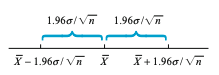
\includegraphics{images/randominterval.png}

}

\end{figure}
\end{frame}

\begin{frame}{Interpreting a Confidence Interval}
\protect\hypertarget{interpreting-a-confidence-interval}{}
The confidence interval defined was inherited from the probability for
the random interval. How can this 95\% confidence interval be
interpreted?
\end{frame}

\begin{frame}{Interpreting a Confidence Interval}
\protect\hypertarget{interpreting-a-confidence-interval-1}{}
We started with the probability that the random interval would capture
the true value of \(\mu\) being 0.95, but then we used data to compute a
fixed interval. Be careful, it is tempting to conclude that \(\mu\) is
within this fixed interval with probability 0.95, but by substituting
\(\bar{x}\) for \(\bar{X}\), all randomness disappears. Therefore, our
calculated interval is not random, and it is thus incorrect to say the
probability \(\mu\) lies in the interval is 0.95.
\end{frame}

\begin{frame}{Interpreting a Confidence Interval}
\protect\hypertarget{interpreting-a-confidence-interval-2}{}
A correct interpretation of ``95\% confidence'' relies on the long-run
relative frequency interpretation of probability: To say that an event A
has probability 0.95 is to say that if the experiment on which A is
defined is performed over and over again, in the long run A will occur
95\% of the time.
\end{frame}

\begin{frame}{Interpreting a Confidence Interval}
\protect\hypertarget{interpreting-a-confidence-interval-3}{}
Let A be the event that
\(\bar{X} - 1.96\cdot \sigma/\sqrt{n} < \mu < \bar{X} + 1.96\cdot \sigma/\sqrt{n}\)
. Since P(A) = 0.95, in the long run 95\% of our computed CIs will
contain \(\mu\). This is illustrated below where the vertical line cuts
the measurement axis at the true (but unknown) value of \(\mu\). Notice
that of the 11 intervals pictured, only intervals 3 and 11 fail to
contain \(\mu\). In the long run, only 5\% of the intervals so
constructed would fail to contain \(\mu\).
\end{frame}

\begin{frame}{Interpreting a Confidence Interval}
\protect\hypertarget{interpreting-a-confidence-interval-4}{}
\begin{figure}

{\centering 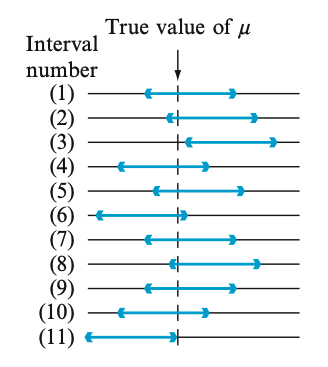
\includegraphics{images/CIinterpretation.png}

}

\end{figure}
\end{frame}

\begin{frame}{Exercise 4}
\protect\hypertarget{exercise-4}{}
A CI is desired for the true average stray-load loss \(\mu\) (watts) for
a certain type of induction motor when the line current is held at 10
amps for a speed of 1,500 rpm. Assume that stray-load loss is normally
distributed with \(\sigma = 3.0\).

\begin{enumerate}[<+->]
[a.]
\tightlist
\item
  Compute a 95\% CI for \(\mu\) when \(n = 25\)\% and
  \(\bar{x} = 58.3\).
\end{enumerate}

\[
\begin{aligned}
\bar{x} -  1.96\cdot \sigma/\sqrt{n} < &\mu < \bar{x} + 1.96\cdot \sigma/\sqrt{n} \\
58.3 -  1.96\cdot 3.0/\sqrt{25} < &\mu < 58.3 1.96\cdot 3.0/\sqrt{25} \\
57.124 < \mu < 59.476
\end{aligned}
\]

Therefore, we are 95\% confident that the true mean stray load loss is
between 57.124 and 59.476 watts.
\end{frame}

\begin{frame}{Exercise 4}
\protect\hypertarget{exercise-4-1}{}
\begin{enumerate}[<+->]
[a.]
\setcounter{enumi}{1}
\tightlist
\item
  Compute a 95\% CI for \(\mu\) when n=100 and \(\bar{x} = 58.3\).
\end{enumerate}
\end{frame}

\begin{frame}{Other Levels of Confidence}
\protect\hypertarget{other-levels-of-confidence}{}
The confidence level of 95\% was inherited from the probability 0.95 for
the initial inequalities. If a confidence level of 99\% was desired
instead,the initial probability of 0.95 must be replaced by 0.99, which
necessitates changing the \(z\) critical value from 1.96 to 2.58. A 99\%
CI then results from using 2.58 in place of 1.96 in the formula for the
95\% CI.
\end{frame}

\begin{frame}{Other Levels of Confidence}
\protect\hypertarget{other-levels-of-confidence-1}{}
We can do this for any desired level of confidence. That is, replace
1.96 or 2.58 with the appropriate standard normal critical value. As the
figure below shows, a probability of \(1-\alpha\) is achieved by using
\(z_{\alpha/2}\) in place of 1.96.

\begin{figure}

{\centering 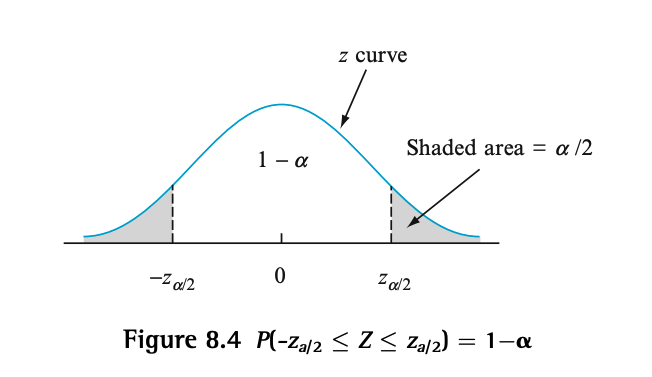
\includegraphics{images/confidencelevel.png}

}

\end{figure}
\end{frame}

\begin{frame}{CIs with Other Levels of Confidence}
\protect\hypertarget{cis-with-other-levels-of-confidence}{}
\begin{tcolorbox}[enhanced jigsaw, titlerule=0mm, colbacktitle=quarto-callout-important-color!10!white, opacityback=0, bottomrule=.15mm, colback=white, colframe=quarto-callout-important-color-frame, arc=.35mm, title=\textcolor{quarto-callout-important-color}{\faExclamation}\hspace{0.5em}{Definition}, toprule=.15mm, breakable, coltitle=black, leftrule=.75mm, bottomtitle=1mm, left=2mm, rightrule=.15mm, toptitle=1mm, opacitybacktitle=0.6]

A \textbf{100(1-}\(\alpha\))\% confidence interval for the mean \(\mu\)
of a normal population when the value of \(\sigma\) is known is given by

\[
\left(\bar{x} - z_{\alpha/2}\cdot\frac{\sigma}{\sqrt{n}}, \bar{x} + z_{\alpha/2}\cdot\frac{\sigma}{\sqrt{n}}\right)
\]

or equivalently, by
\(\bar{x} \pm z_{\alpha/2}\cdot\frac{\sigma}{\sqrt{n}}\).

\end{tcolorbox}
\end{frame}

\begin{frame}{Exercise 4}
\protect\hypertarget{exercise-4-2}{}
A CI is desired for the true average stray-load loss \(\mu\) (watts) for
a certain type of induction motor when the line current is held at 10
amps for a speed of 1,500 rpm. Assume that stray-load loss is normally
distributed with \(\sigma = 3.0\).

\begin{enumerate}[<+->]
[a.]
\setcounter{enumi}{2}
\tightlist
\item
  Compute a 99\% confidence CI for \(\mu\) when \(n=100\) and
  \(\bar{x} = 58.3\).
\end{enumerate}

\[ 
\begin{aligned}
(\bar{x} - z_{\alpha/2} \cdot \frac{\sigma}{\sqrt{n}} &, \bar{x} + z_{\alpha/2} \cdot \frac{\sigma}{\sqrt{n}}) \\
(58.3 - z_{0.005} \cdot \frac{3.0}{\sqrt{100}} &, 58.3 + z_{0.005} \cdot \frac{3.0}{\sqrt{100}})  \\
(58.3 - 2.58 \cdot \frac{3.0}{\sqrt{100}} &, 58.3 + 2.58 \cdot \frac{3.0}{\sqrt{100}} ) \\
(57.526 &, 59.074) \\
\end{aligned}
\]
\end{frame}

\begin{frame}{Exercise 4}
\protect\hypertarget{exercise-4-3}{}
\begin{enumerate}[<+->]
[a.]
\setcounter{enumi}{3}
\tightlist
\item
  Compute an 82\% CI for \(\mu\) when \(n=100\), and \(\bar{x} = 58.3\).
\end{enumerate}
\end{frame}

\begin{frame}{Confidence Level, Precision, and Choice of Sample Size}
\protect\hypertarget{confidence-level-precision-and-choice-of-sample-size}{}
Why settle for a 95\% confidence level when 99\% is achievable?

\begin{itemize}[<+->]
\tightlist
\item
  Because the price paid for a higher confidence level is a wider
  interval!
\item
  As confidence level goes up, so does the width of the interval.
\item
  In fact, the only 100\% CI is \((-\infty,\infty)\).
\item
  If we consider the width of the interval as its precision or accuracy,
  then the confidence level (or reliability) is inversely related to
  precision.
\item
  Thus, a gain in reliability entails a loss in precision.
\item
  How do we handle this?
\end{itemize}
\end{frame}

\begin{frame}{Confidence Level, Precision, and Choice of Sample Size}
\protect\hypertarget{confidence-level-precision-and-choice-of-sample-size-1}{}
An appealing strategy is to specify both the desired confidence level
and interval width and then determine the necessary sample size.

Since the width of an interval is
\(w = 2\cdot z_{\alpha/2}\cdot \sigma/\sqrt{n}\), we can rearrange to
solve for \(n\), the sample size.

\begin{tcolorbox}[enhanced jigsaw, titlerule=0mm, colbacktitle=quarto-callout-important-color!10!white, opacityback=0, bottomrule=.15mm, colback=white, colframe=quarto-callout-important-color-frame, arc=.35mm, title=\textcolor{quarto-callout-important-color}{\faExclamation}\hspace{0.5em}{Formula}, toprule=.15mm, breakable, coltitle=black, leftrule=.75mm, bottomtitle=1mm, left=2mm, rightrule=.15mm, toptitle=1mm, opacitybacktitle=0.6]

\[
n \geq \left(2z_{\alpha/2}\cdot \frac{\sigma}{w} \right)^{2} 
\]

\end{tcolorbox}
\end{frame}

\begin{frame}{Confidence Level, Precision, and Choice of Sample Size}
\protect\hypertarget{confidence-level-precision-and-choice-of-sample-size-2}{}
\begin{itemize}[<+->]
\tightlist
\item
  The smaller the desired width, the large \(n\) must be.
\item
  \(n\) is also an increasing function of \(\sigma\), and of the
  confidence level 100(1-\(\alpha\)).
\item
  The halfwidth of the interval is sometimes called the \textbf{bound on
  the error of estimation} or the \textbf{margin of error}.
\end{itemize}
\end{frame}

\begin{frame}{Example 4}
\protect\hypertarget{example-4}{}
A CI is desired for the true average stray-load loss \(\mu\) (watts) for
a certain type of induction motor when the line current is held at 10
amps for a speed of 1,500 rpm. Assume that stray-load loss is normally
distributed with \(\sigma = 3.0\).

\begin{enumerate}[<+->]
[a.]
\setcounter{enumi}{4}
\tightlist
\item
  How large must \(n\) be if the width of the 99\% interval for \(\mu\)
  is to be 1.0?
\end{enumerate}

\[
\begin{aligned}
n &\geq \left(2z_{\alpha/2}\cdot \frac{\sigma}{w} \right)^{2} \\
&= \left(2\cdot 2.58\cdot \frac{3.0}{1.0} \right)^{2} \\
&= 239.63 \\
\end{aligned} 
\]

Therefore a sample size of 240 is needed to obtain a width of 1.0 at
99\% confidence.
\end{frame}

\begin{frame}{Exercise 5}
\protect\hypertarget{exercise-5}{}
Assume that the helium porosity (in percentage) of coal samples taken
from any particular seam is normally distributed with true standard
deviation 0.75.

\begin{enumerate}[<+->]
[a.]
\setcounter{enumi}{4}
\tightlist
\item
  What sample size is necessary to estimate true average porosity to
  within 0.2 with 99\% confidence?
\end{enumerate}
\end{frame}

\begin{frame}{Deriving a Confidence Interval}
\protect\hypertarget{deriving-a-confidence-interval}{}
Let \(X_{1}\), \(X_{2}\),\ldots,\(X_{n}\) denote the sample on which the
CI for a parameter \(\theta\) is to be based. Suppose a random variable
satisfying the following two properties can be found.

\begin{enumerate}[<+->]
\tightlist
\item
  The variable depends functionally on both \(X_{1}\), \ldots, \(X_{n}\)
  and \(\theta\).
\item
  The probability distribution of the variable does not depend on
  \(\theta\) or on any other unknown parameters.
\end{enumerate}
\end{frame}

\begin{frame}{Deriving a Confidence Interval}
\protect\hypertarget{deriving-a-confidence-interval-1}{}
Let \(h(X_{1}, X_{2}, ... , X_{n}; y)\) denote this random variable. For
example, if the population distribution is normal with known \(\sigma\)
and \(\theta = \mu\), the variable
\(h(X_{1}; ... ; X_{n}; \theta) = (X - \mu)/(\sigma/\sqrt{n})\)
satisfies both properties; it clearly depends functionally on \(\mu\),
yet has the standard normal probability distribution, which does not
depend on \(\mu\). In general, the form of the \(h\) function is usually
suggested by examining the distribution of an appropriate estimator
\(\hat{\theta}\).
\end{frame}

\begin{frame}{Deriving a Confidence Interval}
\protect\hypertarget{deriving-a-confidence-interval-2}{}
For any \(\alpha\) between \(0\) and \(1\), constants \(a\) and \(b\)
can be found to satisfy

\[
P[a < h(X_{1}; ... ; X_{n}; \theta) < b] = 1  - \alpha
\]

Because of the second property, \(a\) and \(b\) do not depend on
\(\theta\). In the normal example \(a = -z_{\alpha/2}\) and
\(b = z_{\alpha/2}\). Now suppose that the inequalities above can be
manipulated to isolate \(\theta\), giving the equivalent probability
statement

\[
P[l(X_{1},...,X_{n}) < \theta < u(X_{1},...,x_{n})] = 1 - \alpha
\]

Then \(l(x_{1}, x_{2}, ... , x_{n})\) and \(u(x_{1}, ... , x_{n})\) are
the lower and upper confidence limits, respectively, for a
\(100(1 - \alpha)\%\) CI. In the normal example, we saw that
\(l(X_{1}, ..., X_{n}) = \bar{X} - z_{\alpha/2} \cdot \sigma/ \sqrt{n}\)
and
\(u(X_{1}, ..., X_{n}) = \bar{X} + z_{\alpha/2} \cdot \sigma/ \sqrt{n}\).
\end{frame}

\begin{frame}{Summary}
\protect\hypertarget{summary}{}
\begin{itemize}[<+->]
\tightlist
\item
  A \textbf{confidence interval} is an interval of plausible values for
  parameter of interest, or an interval estimate of the parameter.
\item
  The \textbf{confidence level} is a measure of the degree of
  reliability of the interval.
\item
  The interpretation of a confidence interval is that if we collect many
  samples of size \(n\) and for each, calculate a (1-\(\alpha\))100\% CI
  for each, then we expect (1-\(\alpha\))100\% of these intervals to
  capture \(\mu\).
\item
  \(z_{\alpha/2}\) is the value on the standard normal distribution that
  has upper area \(\alpha/2\).
\end{itemize}
\end{frame}

\begin{frame}{Summary}
\protect\hypertarget{summary-1}{}
\begin{itemize}[<+->]
\tightlist
\item
  A (1-\(\alpha\))100\% CI for the mean \(\mu\) of a normal population
  when the value of \(\sigma\) is known is given by
\end{itemize}

\[
\bar{x} \pm z_{\alpha/2}\cdot \frac{\sigma}{\sqrt{n}}
\]

\begin{itemize}[<+->]
\tightlist
\item
  To obtain a interval with width \(w\) at a given confidence level
  (\(1-\alpha\))100\% when we know \(\sigma\), we need
\end{itemize}

\[
n \geq \left( 2\cdot z_{\alpha/2}\cdot \frac{\sigma}{w}\right)^{2}
\]

\begin{itemize}[<+->]
\tightlist
\item
  The half width of an interval is called the \textbf{margin of error}.
\end{itemize}
\end{frame}

\begin{frame}{Practice Problems}
\protect\hypertarget{practice-problems}{}
\begin{itemize}[<+->]
\tightlist
\item
  Odd problems 1 - 11
\end{itemize}
\end{frame}

\hypertarget{large-sample-confidence-intervals-for-a-population-mean-and-proportion}{%
\section{8.2 Large-Sample Confidence Intervals for a Population Mean and
Proportion}\label{large-sample-confidence-intervals-for-a-population-mean-and-proportion}}

\begin{frame}{Outcomes}
\protect\hypertarget{outcomes-1}{}
\begin{itemize}[<+->]
\tightlist
\item
  Know how and when to calculate a large-sample interval for \(\mu\).
\item
  Know how and when to calculate a general large-sample confidence
  interval.
\item
  Know how and when to calculate a confidence interval for a population
  proportion using the score CI or the traditional CI, and know the
  benefits of using either.
\item
  Know how and when to use one-sided confidence intervals.
\end{itemize}
\end{frame}

\begin{frame}{Introduction}
\protect\hypertarget{introduction-3}{}
The CI for \(\mu\) presented in the previous section assumed that the
population distribution is normal and that the value of \(\sigma\) is
known. We now present a large-sample CI whose validity does not require
these assumptions.
\end{frame}

\begin{frame}{A Large-Sample Interval for Mean}
\protect\hypertarget{a-large-sample-interval-for-mean}{}
Let \(X_{1}\), \(X_{2}\),\ldots, \(X_{n}\) be a random sample from a
population having a mean \(\mu\) and standard deviation \(\sigma\).
Provided that \(n\) is large, the Central Limit Theorem (CLT) implies
that \(\bar{X}\) has approximately a normal distribution whatever the
nature of the population distribution. It then follows that
\(Z = \frac{\bar{X}-\mu}{\sigma/\sqrt{n}}\) has approximately a standard
normal distribution, so that:

\[
P\left(-z_{\alpha/2} < \frac{\bar{X} - \mu}{\sigma/\sqrt{n}} < z_{\alpha/2}\right) \approx 1 - \alpha
\]
\end{frame}

\begin{frame}{A Large-Sample Interval for Mean}
\protect\hypertarget{a-large-sample-interval-for-mean-1}{}
But this still requires \(\sigma\), which will almost never be known.
Consider the standardized variable

\[
Z = \frac{\bar{X} - \mu}{S/\sqrt{n}}
\]

where \(\sigma\), is replaced by the sample standard deviation \(S\).
Previously there was randomness only in the number of \(Z\), but now
there is randomness in the numerator and the denominator - the values of
both \(\bar{X}\) and \(S\) vary from sample to sample. However, when
\(n\) is large, the use of \(S\) rather than \(\sigma\) adds very little
extra variability to \(Z\). More specifically, in this case the new
\(Z\) also has approximately a standard normal distribution.
\end{frame}

\begin{frame}{A Large-Sample Confidence Interval for Mean}
\protect\hypertarget{a-large-sample-confidence-interval-for-mean}{}
\begin{tcolorbox}[enhanced jigsaw, titlerule=0mm, colbacktitle=quarto-callout-important-color!10!white, opacityback=0, bottomrule=.15mm, colback=white, colframe=quarto-callout-important-color-frame, arc=.35mm, title=\textcolor{quarto-callout-important-color}{\faExclamation}\hspace{0.5em}{Proposition}, toprule=.15mm, breakable, coltitle=black, leftrule=.75mm, bottomtitle=1mm, left=2mm, rightrule=.15mm, toptitle=1mm, opacitybacktitle=0.6]

If \(n\) is sufficiently large, the standardized variable

\[
Z = \frac{\bar{X} - \mu}{S/\sqrt{n}}
\]

has approximately a standard normal distribution. This implies that

\[
\bar{x} \pm z_{\alpha/2}\cdot \frac{s}{\sqrt{n}}
\]

is a \textbf{large-sample confidence interval for} \(\mu\) with
confidence level approximately 100(\(1-\alpha\))\%. This formula is
valid regardless of the shape of the population distribution.

\end{tcolorbox}
\end{frame}

\begin{frame}{A Large-Sample Confidence Interval for Mean}
\protect\hypertarget{a-large-sample-confidence-interval-for-mean-1}{}
Speaking generally, \(n>40\) will be sufficient to justify the use of
this interval. This is somewhat more conservative than the rule of thumb
for the CLT because of the additional variability introduced by using
\(S\) in place of \(\sigma\).
\end{frame}

\begin{frame}{Exercise 12}
\protect\hypertarget{exercise-12}{}
A random sample of 110 lightning flashes in a region resulted in a
sample average radar echo duration of 0.81s and a sample standard
deviation of 0.34 s. Calculate a 99\% confidence interval for the true
average echo duration \(\mu\) and interpret the resulting interval.
\end{frame}

\begin{frame}{Exercise 12 Solutions}
\protect\hypertarget{exercise-12-solutions}{}
\(n = 110\)\\
\(\bar{x} = 0.81\)\\
\(s = 0.34\)\\
\(\alpha = 0.01\)

\[ 
\begin{aligned}
\bar{x} &\pm z_{\alpha/2}\cdot \frac{s}{\sqrt{n}} \\
0.81 &\pm z_{0.005}\cdot \frac{0.34}{\sqrt{110}} \\
0.81 &\pm 2.575 \cdot \frac{0.34}{\sqrt{110}} \\
0.81 &\pm 0.083 \\
(0.727&, 0.893)
\end{aligned}
\]

We are 99\% confident that the true average radar echo duration of
lightning flashes in a region is between 0.727 and 0.893 MPa.
\end{frame}

\begin{frame}{Exercise 14}
\protect\hypertarget{exercise-14}{}
An article gave the following summary information for fracture strengths
(MPa) of \(n = 169\) ceramic bars fired in a particular kiln:
\(\bar{x} = 89.10, s = 3.73\).

\begin{enumerate}[<+->]
[a.]
\tightlist
\item
  Calculate a (two-sided) confidence interval for true average fracture
  strength using a confidence level of 95\%. Does it appear that true
  average fracture strength has been precisely estimated?
\item
  Suppose the investigators had believed a priori that the population
  standard deviation was about 4 MPa. Based on this supposition, how
  large a sample would have been required to estimate \(\mu\) to within
  0.5 MPa with 95\% confidence?
\end{enumerate}
\end{frame}

\begin{frame}{A General Large-Sample Confidence Interval}
\protect\hypertarget{a-general-large-sample-confidence-interval}{}
Suppose that \(\hat{\theta}\) is an estimator satisfying the following
properties:

\begin{enumerate}[<+->]
\tightlist
\item
  It has approximately a normal distribution.
\item
  It is (at least approximately) unbiased.
\item
  An expression for \(\sigma_{\hat{\theta}}\), the standard deviation of
  \(\hat{\theta}\) is available.
\end{enumerate}

For example, in the case of \(\theta = \mu\), \(\hat{\mu} = \bar{X}\) is
an unbiased estimator whose distribution is approximately normal when
\(n\) is large and
\(\sigma_{\hat{\mu}} = \sigma_{\bar{X}} = \sigma/\sqrt{n}\).
Standardizing \(\hat{\theta}\) yields the rv
\(Z = (\hat{\theta} - \theta)/\sigma_{\hat{\theta}}\), which has
approximately a standard normal distribution. This justifies the
probability statement

\[
P\left(-z_{\alpha/2} < \frac{\hat{\theta} - \theta}{\sigma_{\hat{\theta}}} < z_{\alpha/2}\right) \approx 1 - \alpha
\]
\end{frame}

\begin{frame}{A General Large-Sample Confidence Interval}
\protect\hypertarget{a-general-large-sample-confidence-interval-1}{}
Finally, suppose that \(\sigma_{\hat{\theta}}\) does involve the unknown
\(\sigma\). This is the case, for example, when \(\theta=p\), a
population proportion. Then
\((\hat{\theta} - \theta)/\sigma_{\hat{\theta}} = z_{\alpha/2}\) can be
difficult to solve. An approximate solution can often be obtained by
replacing \(\theta\) in \(\sigma_{\hat{\theta}}\) by its estimate
\(\hat{\theta}\). This results in an estimated standard deviation
\(s_{\hat{\theta}}\), and the corresponding interval is again
\(\hat{\theta} \pm z_{\alpha/2}\cdot s_{\hat{\theta}}\)
\end{frame}

\begin{frame}{Exercise 26}
\protect\hypertarget{exercise-26}{}
The superintendent of a large school district, having once had a course
in probability and statistics, believes that the number of teachers
absent on any given day has a Poisson distribution with parameter
\(\lambda\). Use the accompanying data on absences for 50 days to derive
a large-sample CI for \(\lambda\). {[}Hint: The mean and variance of a
Poisson variable both equal \(\lambda\){]}, so

\[
Z = \frac{\bar{X} - \lambda}{\sqrt{\lambda/n}}
\]

has approximately a standard normal distribution. Make a probability
statement (with probability 1 - \(\alpha\)) and solve the resulting
inequalities for \(\lambda\).

\begin{longtable}[]{@{}
  >{\raggedright\arraybackslash}p{(\columnwidth - 22\tabcolsep) * \real{0.2667}}
  >{\raggedright\arraybackslash}p{(\columnwidth - 22\tabcolsep) * \real{0.0667}}
  >{\raggedright\arraybackslash}p{(\columnwidth - 22\tabcolsep) * \real{0.0667}}
  >{\raggedright\arraybackslash}p{(\columnwidth - 22\tabcolsep) * \real{0.0667}}
  >{\raggedright\arraybackslash}p{(\columnwidth - 22\tabcolsep) * \real{0.0667}}
  >{\raggedright\arraybackslash}p{(\columnwidth - 22\tabcolsep) * \real{0.0667}}
  >{\raggedright\arraybackslash}p{(\columnwidth - 22\tabcolsep) * \real{0.0667}}
  >{\raggedright\arraybackslash}p{(\columnwidth - 22\tabcolsep) * \real{0.0667}}
  >{\raggedright\arraybackslash}p{(\columnwidth - 22\tabcolsep) * \real{0.0667}}
  >{\raggedright\arraybackslash}p{(\columnwidth - 22\tabcolsep) * \real{0.0667}}
  >{\raggedright\arraybackslash}p{(\columnwidth - 22\tabcolsep) * \real{0.0667}}
  >{\raggedright\arraybackslash}p{(\columnwidth - 22\tabcolsep) * \real{0.0667}}@{}}
\toprule()
\begin{minipage}[b]{\linewidth}\raggedright
Number of absences
\end{minipage} & \begin{minipage}[b]{\linewidth}\raggedright
0
\end{minipage} & \begin{minipage}[b]{\linewidth}\raggedright
1
\end{minipage} & \begin{minipage}[b]{\linewidth}\raggedright
2
\end{minipage} & \begin{minipage}[b]{\linewidth}\raggedright
3
\end{minipage} & \begin{minipage}[b]{\linewidth}\raggedright
4
\end{minipage} & \begin{minipage}[b]{\linewidth}\raggedright
5
\end{minipage} & \begin{minipage}[b]{\linewidth}\raggedright
6
\end{minipage} & \begin{minipage}[b]{\linewidth}\raggedright
7
\end{minipage} & \begin{minipage}[b]{\linewidth}\raggedright
8
\end{minipage} & \begin{minipage}[b]{\linewidth}\raggedright
9
\end{minipage} & \begin{minipage}[b]{\linewidth}\raggedright
10
\end{minipage} \\
\midrule()
\endhead
Frequency & 1 & 4 & 8 & 10 & 8 & 7 & 5 & 3 & 2 & 1 & 1 \\
\bottomrule()
\end{longtable}
\end{frame}

\begin{frame}{Exercise 26 Solutions}
\protect\hypertarget{exercise-26-solutions}{}
\[
P(-z_{\alpha/2} < \frac{\bar{X} - \lambda}{\sqrt{\lambda/n}} < z_{\alpha/2} ) \approx 1 - \alpha 
\]

Now we need to rearrange the inequality in the probability statement to
solve for \(\lambda\). Let's consider it as an equality statement first
for simplicity.

\[
\begin{aligned}
\frac{\bar{X} - \lambda}{\sqrt{\lambda/n}} &= \pm z_{\alpha/2}\\
\bar{X} - \lambda &= \pm z_{\alpha/2}\sqrt{\lambda/n} \\
(\bar{X} - \lambda)^{2} &= (\pm z_{\alpha/2}\sqrt{\lambda/n})^{2} \\
\bar{X}^{2} -2\bar{X}\lambda + \lambda^{2} &= z_{\alpha/2}^{2}\lambda/n \\
\bar{X}^{2} -(2\bar{X} + z^{2}_{\alpha/2}/n)\lambda + \lambda^{2} &= 0 
\end{aligned}
\]
\end{frame}

\begin{frame}{Exercise 26 Solutions}
\protect\hypertarget{exercise-26-solutions-1}{}
From the quadratic equation, letting \(a = 1\),
\(b = -(2\bar{X} + z^{2}_{\alpha/2}/n)\) and \(c = \bar{X}^{2}\).

\[
\begin{aligned}
\frac{-b \pm \sqrt{b^{2} - 4ac}}{2a} \\
\frac{-(-(2\bar{X} + z^{2}_{\alpha/2}/n)) \pm \sqrt{[-(2\bar{X} + z^{2}_{\alpha/2}/n)]^{2} - 4\bar{X}^{2}}}{2} \\
\bar{X} + \frac{z^{2}_{\alpha/2}}{2n} \pm \frac{\sqrt{4\bar{X}^{2} + 4\bar{X}z_{\alpha/2}^{2}/n + z_{\alpha/2}^{4}/n^{2} - 4\bar{X}^{2}}}{2} \\
\bar{X} + \frac{z^{2}_{\alpha/2}}{2n} \pm \frac{\sqrt{4\bar{X}z_{\alpha/2}^{2}/n + z_{\alpha/2}^{4}/n^{2}}}{2} \\
\bar{X} + \frac{z^{2}_{\alpha/2}}{2n} \pm z_{\alpha/2}\frac{\sqrt{4n\bar{X} + z_{\alpha/2}^{2}}}{2n} 
\end{aligned}
\]
\end{frame}

\begin{frame}{Exercise 26 Solutions}
\protect\hypertarget{exercise-26-solutions-2}{}
Therefore, we can plug into the final statement to obtain our confidence
bounds for \(\lambda\).

From the data, we get that \(\bar{X} = 203/50 = 4.06\), \(n=50\) and for
95\% confidence, \(z_{0.025} = 1.96\).
\end{frame}

\begin{frame}{Exercise 26 Solutions}
\protect\hypertarget{exercise-26-solutions-3}{}
\[
\begin{aligned}
\bar{X} + \frac{z^{2}_{\alpha/2}}{2n} &\pm z_{\alpha/2}\frac{\sqrt{4n\bar{X} + z_{\alpha/2}^{2}}}{2n} \\
4.06 + \frac{1.96^{2}}{2(50)} &\pm 1.96\frac{\sqrt{4(50)(4.06) + 1.96^{2}}}{2(50)} \\
4.0984 &\pm 1.96\frac{\sqrt{815.8416}}{100} \\
4.0984 &\pm 0.5598\\
(3.5386&, 4.6582)
\end{aligned}
\]
\end{frame}

\begin{frame}{Exercise 26 Solution}
\protect\hypertarget{exercise-26-solution}{}
Note that for large \(n\), this is approximately equivalent to
\(\bar{X} \pm z_{\alpha/2}\frac{\sqrt{\bar{X}}}{\sqrt{n}} = \hat{\mu} \pm z_{\alpha/2}\frac{\hat{\sigma}}{\sqrt{n}}\)
(since \(\mu= \sigma^{2} = \lambda\) for the Poisson distribution).
\end{frame}

\begin{frame}{A Confidence Interval for a Population Proportion}
\protect\hypertarget{a-confidence-interval-for-a-population-proportion}{}
\begin{itemize}[<+->]
\tightlist
\item
  Let \(p\) denote the proportion of ``successes'' in a population,
  where success identifies an individual of object that has a specified
  property.
\item
  A random sample of \(n\) individuals is to be selected, and \(X\) is
  the number of successes in the sample.
\item
  Provided that \(n\) is small compared to the population size, \(X\)
  can be regarded as a binomial random variable with \(E(X) = np\) and
  \(\sigma_{X} = \sqrt{np(1-p)}\).
\item
  Furthermore, if \(n\) is large, (\(np \geq 10\) and \(nq \geq 10\)),
  \(X\) has approximately a normal distribution.
\end{itemize}
\end{frame}

\begin{frame}{A Confidence Interval for a Population Proportion}
\protect\hypertarget{a-confidence-interval-for-a-population-proportion-1}{}
\begin{itemize}[<+->]
\tightlist
\item
  The natural estimator of \(p\) is \(\hat{p} = X/n\), the sample
  fraction of successes.
\item
  Since \(\hat{p}\) is just \(X\) multiplied by a constant, \(\hat{p}\)
  also has approximately a normal distribution.
\item
  As shown in Section 7.1, \(E(\hat{p}) = p\) (unbiasedness) and
  \(\sigma_{\hat{p}} = \sqrt{p(1-p)/n}\).
\item
  The standard deviation \(\sigma_{\hat{p}}\) involves the unknown
  parameter \(p\). Standardizing \(\hat{p}\) by subtracting \(p\) and
  dividing by \(\sigma_{\hat{p}}\) then implies that:
\end{itemize}

\[
P(-z_{\alpha/2} < \frac{\hat{p} - p}{\sqrt{p(1-p)/n}} < z_{\alpha/2}) \approx 1-\alpha
\]

\textbf{Show derivation on board}
\end{frame}

\begin{frame}{A Confidence Interval for a Population Proportion}
\protect\hypertarget{a-confidence-interval-for-a-population-proportion-2}{}
\begin{tcolorbox}[enhanced jigsaw, titlerule=0mm, colbacktitle=quarto-callout-important-color!10!white, opacityback=0, bottomrule=.15mm, colback=white, colframe=quarto-callout-important-color-frame, arc=.35mm, title=\textcolor{quarto-callout-important-color}{\faExclamation}\hspace{0.5em}{Proposition}, toprule=.15mm, breakable, coltitle=black, leftrule=.75mm, bottomtitle=1mm, left=2mm, rightrule=.15mm, toptitle=1mm, opacitybacktitle=0.6]

Let
\(\tilde{p} = \frac{\hat{p} + z_{\alpha/2}^{2}/2n}{1 + z^{2}_{\alpha/2}/n}\).
Then a \textbf{confidence interval for a population proportion p} with
confidence level approximately 100(1-\(\alpha\))\% is

\[
\tilde{p} \pm z_{\alpha/2}\frac{\sqrt{\hat{p}\hat{q}/n + z_{\alpha/2}^{2}/4n^{2}}}{1+z^{2}_{\alpha/2}/n}
\]

where \(\hat{q} = 1 - \hat{p}\). This is often referred to the ``score
CI'' for \(p\).

\end{tcolorbox}
\end{frame}

\begin{frame}{Exercise 20}
\protect\hypertarget{exercise-20}{}
The Associated Press (October 9, 2002) reported that in a survey of 4722
American youngsters aged 6-19, 15\% were seriously overweight (a body
mass index of at least 30; this index is a measure of weight relative to
height). Calculate and interpret a confidence interval using a 99\%
confidence level for the proportion of all American youngsters who are
seriously overweight.
\end{frame}

\begin{frame}{Exercise 20 Solutions}
\protect\hypertarget{exercise-20-solutions}{}
\(\hat{p} = 0.15\)\\
\(n = 4722\)\\
\(z_{\alpha/2} = z_{0.005} = 2.575\).

\[ 
\begin{aligned}
\tilde{p} &= \frac{\hat{p} + z_{\alpha/2}^{2}/2n}{1 + z^{2}_{\alpha/2}/n} \\
&= \frac{0.15 + 2.575^{2}/2(4722)}{1 + 2.575^{2}/4722} \\
&= 0.1505
\end{aligned}
\]
\end{frame}

\begin{frame}{Exercise 20 Solutions}
\protect\hypertarget{exercise-20-solutions-1}{}
\[
\begin{aligned}
\tilde{p} &\pm z_{\alpha/2}\frac{\sqrt{\hat{p}\hat{q}/n + z_{\alpha/2}^{2}/4n^{2}}}{1+z^{2}_{\alpha/2}/n} \\
0.1505 &\pm 2.575\frac{\sqrt{0.15(0.85)/4722 + 2.575^{2}/4(4722)^{2}}}{1+2.575^{2}/4722} \\
0.1505 &\pm 0.0134 \\
(0.1371&, 0.1639)
\end{aligned}
\]
\end{frame}

\begin{frame}{Example 1}
\protect\hypertarget{example-1}{}
An insurance company checks police records on 582 accidents selected at
random and notes that teenagers were at the wheel in 91 of them.

\begin{enumerate}[<+->]
[a.]
\tightlist
\item
  Create a 95\% confidence interval for the percentage of all auto
  accidents that involve teenage drivers.
\item
  Explain what your interval means.
\item
  Explain what ``95\% confidence'' means.
\item
  A politician urging tight restrictions on drivers' licenses issued to
  teens says, ``In one of every five auto accidents, a teenager is
  behind the wheel.'' Does your confidence interval support or
  contradict this statement?
\end{enumerate}
\end{frame}

\begin{frame}{Large n}
\protect\hypertarget{large-n}{}
\begin{itemize}[<+->]
\item
  If the sample size \(n\) is very large, then \(z_{\alpha/2}^{2}/2n\)
  is generally quite small compared to \(\hat{p}\), and
  \(z_{\alpha/2}^{2}/n\) is quite small compared to 1. Therefore,
  \(\tilde{p} \approx \hat{p}\).
\item
  Similarly, \(z_{\alpha/2}^{2}/4n^{2}\) is small compared to
  \(\hat{p}\hat{q}/n\) and so the dominant term in the \(\pm\)
  expression is \(z_{\alpha/2}\sqrt{\hat{p}\hat{q}/n}\) and the score
  interval is approximately
\end{itemize}

\[ 
\hat{p} \pm z_{\alpha/2}\sqrt{\hat{p}\hat{q}/n}
\]

\begin{itemize}[<+->]
\tightlist
\item
  Note, this has the general form
  \(\hat{\theta} \pm z_{\alpha/2}\hat{\sigma}_{\theta}\) of a
  large-sample interval suggested in the last subsection.
\end{itemize}
\end{frame}

\begin{frame}{How large is large?}
\protect\hypertarget{how-large-is-large}{}
\begin{itemize}[<+->]
\tightlist
\item
  So how large of an \(n\) do we need?
\item
  To use this traditional interval, we need to check that:
\end{itemize}

\[
n\hat{p} \geq 10 \& n(1-\hat{p}) \geq 10
\]
\end{frame}

\begin{frame}{So Why Bother?}
\protect\hypertarget{so-why-bother}{}
First, let's introduce two terms:

\begin{itemize}[<+->]
\tightlist
\item
  \textbf{nominal confidence level}: the one we think that we have by
  using the z critical value.
\item
  \textbf{coverage probability}: the probability that a random interval
  includes the actual value of \(p\).
\end{itemize}

The actual coverage probability can differ greatly from the nominal
probability, particularly when \(p\) is not close to 0.5.
\end{frame}

\begin{frame}{Nominal level vs Coverage Probability}
\protect\hypertarget{nominal-level-vs-coverage-probability}{}
\begin{figure}

{\centering 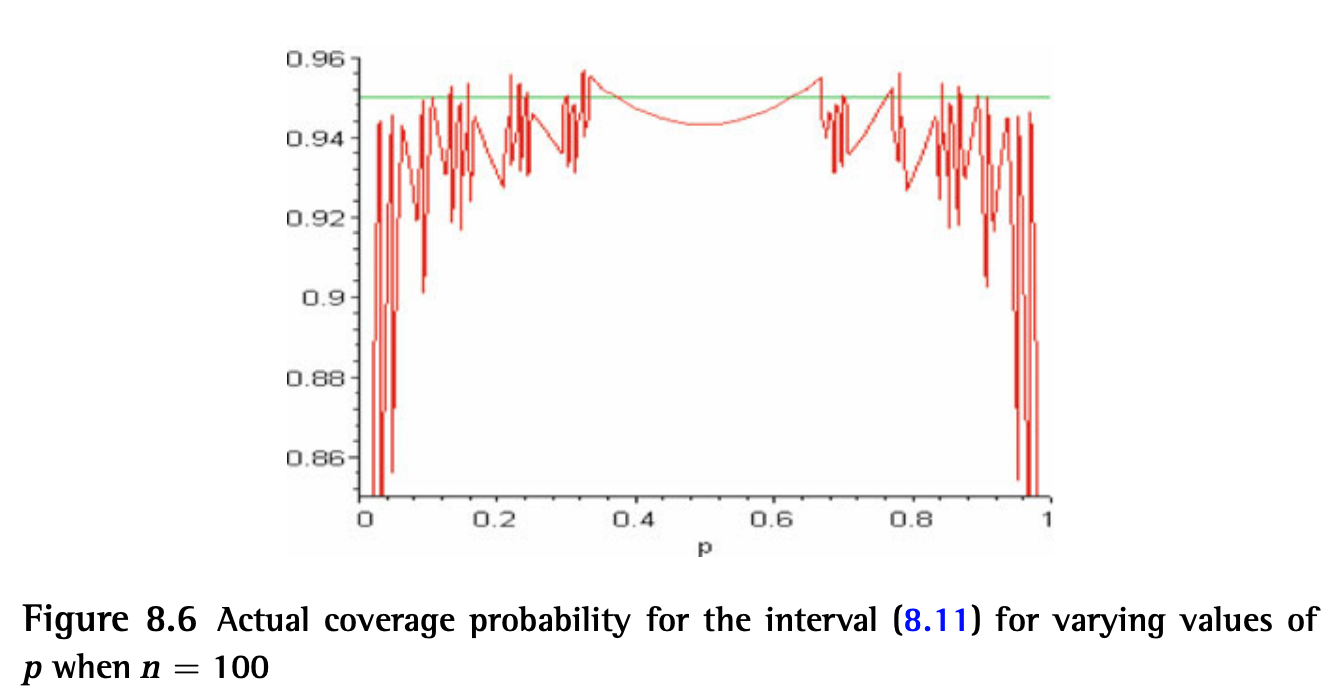
\includegraphics{images/nominal.png}

}

\end{figure}
\end{frame}

\begin{frame}{Score Interval vs Traditional Interval}
\protect\hypertarget{score-interval-vs-traditional-interval}{}
With the traditional interval, the nominal probability (0.95 in the
graph) can differ greatly from the actual coverage probability, even for
reasonably large sample sizes. The score interval rectifies this
behaviour. That is, it's actual coverage probability will be quite close
to the nominal level specified by \(z_{\alpha/2}\).

Additionally, the score interval can be used with nearly all sample
sizes and parameter values. Therefore, we do not have to check that
\(n\hat{p} \geq 10\) and \(n(1-\hat{p}) \geq 10\), which is required
when the traditional interval is used.
\end{frame}

\begin{frame}{Exercise 20}
\protect\hypertarget{exercise-20-1}{}
Use the traditional interval.

The Associated Press (October 9, 2002) reported that in a survey of 4722
American youngsters aged 6-19, 15\% were seriously overweight (a body
mass index of at least 30; this index is a measure of weight relative to
height). Calculate and interpret a confidence interval using a 99\%
confidence level for the proportion of all American youngsters who are
seriously overweight.
\end{frame}

\begin{frame}{Exercise 20 Solutions}
\protect\hypertarget{exercise-20-solutions-2}{}
\(\hat{p} = 0.15\)\\
\(n = 4722\)\\
\(z_{\alpha/2} = z_{0.005} = 2.575\).

First, check!

\[
\begin{aligned}
n\hat{p} &= 4722(0.15) \\
&= 708.3 \geq 10
\end{aligned}
\]

\[
\begin{aligned}
n(1-\hat{p}) &= 4722(1-0.15) \\
&= 4013.7 \geq 10
\end{aligned}
\]
\end{frame}

\begin{frame}{Exercise 20 Solutions}
\protect\hypertarget{exercise-20-solutions-3}{}
\[ 
\begin{aligned}
\hat{p} &\pm z_{\alpha/2}\sqrt{\hat{p}\hat{q}/n} \\
0.15 &\pm 2.575\sqrt{(0.15)(0.85)/4722}\\
0.15 &\pm 0.0134 \\
(0.1355&, 0.1634)
\end{aligned}
\]

Therefore, we are 99\% confidence that the proportion of all American
youngsters who are seriously overweight is between 0.1355 and 0.1634.
\end{frame}

\begin{frame}{Example 2}
\protect\hypertarget{example-2}{}
An insurance company checks police records on 582 accidents selected at
random and notes that teenagers were at the wheel in 91 of them.

Use 95\% confidence and the traditional interval and compare to the
score interval found earlier.
\end{frame}

\begin{frame}{One-Sided Confidence Intervals (Confidence Bounds)}
\protect\hypertarget{one-sided-confidence-intervals-confidence-bounds}{}
\begin{itemize}[<+->]
\tightlist
\item
  So far, we have discussed ways of calculating confidence bounds where
  there is both an upper and a lower bound.
\item
  Sometimes, an investigator will only want one of these two bounds.
\item
  For example, a psychologist may wish to calculate a 95\% upper
  confidence bound for true average reaction time to a particular
  stimulus, or a surgeon may want only a lower confidence bound for the
  true average remission time after colon cancer surgery.
\end{itemize}

\[
P\left( \frac{\bar{X} - \mu}{S/\sqrt{n}} < z_{\alpha}\right) 1 - \alpha
\]

Manipulating the inequality, we get the results on the following slide.
\end{frame}

\begin{frame}{One-Sided Confidence Intervals (Confidence Bounds)}
\protect\hypertarget{one-sided-confidence-intervals-confidence-bounds-1}{}
\begin{tcolorbox}[enhanced jigsaw, titlerule=0mm, colbacktitle=quarto-callout-important-color!10!white, opacityback=0, bottomrule=.15mm, colback=white, colframe=quarto-callout-important-color-frame, arc=.35mm, title=\textcolor{quarto-callout-important-color}{\faExclamation}\hspace{0.5em}{Proposition}, toprule=.15mm, breakable, coltitle=black, leftrule=.75mm, bottomtitle=1mm, left=2mm, rightrule=.15mm, toptitle=1mm, opacitybacktitle=0.6]

A \textbf{large-sample upper confidence bound for} \(\boldsymbol\mu\) is

\[
\mu < \bar{x} + z_{\alpha} \frac{s}{\sqrt{n}}
\]

and a \textbf{large-sample lower confidence bound for}
\(\boldsymbol\mu\) is

\[
\mu > \bar{x} - z_{\alpha} \frac{s}{\sqrt{n}}
\]

A \textbf{one-sided confidence bound for p} results from replacing
\(z_{\alpha/2}\) by \(z_{\alpha}\) and \(\pm\) by either \(+\) or \(-\)
in the CI formula for \(p\). In all cases, the confidence level is
approximately \(100(1-\alpha)\)\%.

\end{tcolorbox}
\end{frame}

\begin{frame}{Exercise 16}
\protect\hypertarget{exercise-16}{}
A sample of 66 obese adults as put on a low-carbohydrate diet for a
year. The average weight loss was 11 lb and the standard deviation was
19 lb. Calculate a 99\% lower confidence bound for the true average
weight loss. What does this bound say about confidence that that the
mean weight loss is positive?
\end{frame}

\begin{frame}{Exercise 16 Solutions}
\protect\hypertarget{exercise-16-solutions}{}
\(n = 66\)\\
\(\bar{x} = 11\)\\
\(s = 19\)\\
\(z_{0.01} = 2.33\)

\[
\begin{aligned}
\mu &> \bar{x} - z_{\alpha}\frac{s}{\sqrt{n}} \\ 
&> 11 - 2.33 \frac{19}{\sqrt{66}} \\ 
&> 5.55
\end{aligned}
\]

Therefore, we are 99\% confident that the true average weight loss of
all adults put on a low-carbohydrate diet for a year is larger than 5.55
lbs. So, we are very certain that \(\mu\) is positive.
\end{frame}

\begin{frame}{Exercise 22}
\protect\hypertarget{exercise-22}{}
In a sample of 1000 randomly selected consumers who had opportunities to
send in a rebate claim form after purchasing a product, 250 of these
people said they never did so. Reasons cited for their behaviour
included too many steps in the process, amount too small, missed
deadline, fear of being placed on a mailing list, lost receipt, and
doubts about receiving the money. Calculate an upper confidence bound at
the 95\% level for the true proportion of such consumers who never apply
for a rebate. Based on this bound, is there compelling evidence that the
true proportion of such consumers is smaller than 1/3?. Explain your
reasoning.
\end{frame}

\begin{frame}{Summary}
\protect\hypertarget{summary-2}{}
\begin{itemize}[<+->]
\tightlist
\item
  A large-sample CI for \(\mu\) is calculated by
  \(\bar{x} \pm z_{\alpha/2}\cdot \frac{s}{\sqrt{n}}\) for
  \(100(1-\alpha)\)\% confidence when \(n\) is sufficiently large
  (\(n>40\)).
\item
  If the estimator is approximately normally distributed and
  approximately unbiased, and n is sufficiently large, then
  \(\hat{\theta} \pm z_{\alpha/2}\cdot s_{\hat{\theta}}\) is a general
  large-sample confidence interval with confidence \(100(1-\alpha)\)\%.
\item
  The score CI for \(p\) is given by
  \(\tilde{p} \pm z_{\alpha/2}\frac{\sqrt{\hat{p}\hat{q}/n + z_{\alpha/2}^{2}/4n^{2}}}{1+z^{2}_{\alpha/2}/n}\)
  where \(\hat{q} = 1 - \hat{p}\) and
  \(\tilde{p} = \frac{\hat{p} + z_{\alpha/2}^{2}/2n}{1 + z^{2}_{\alpha/2}/n}\).
\end{itemize}
\end{frame}

\begin{frame}{Summary}
\protect\hypertarget{summary-3}{}
\begin{itemize}[<+->]
\tightlist
\item
  The traditional CI for \(p\) is given by
  \(\hat{p} \pm z_{\alpha/2}\sqrt{\hat{p}\hat{q}/n}\). When \(p\) is
  close to 0.5, the traditional CI is okay to use, however, when \(p\)
  is close to 0 or 1, the score CI is preferred.
\item
  One sided confidence bounds can be found by replacing \(z_{\alpha/2}\)
  with \(z_{\alpha}\) and using either \(+\) or \(-\) in place of
  \(\pm\) depending on if we want the upper or lower confidence bound.
\end{itemize}
\end{frame}

\begin{frame}{Practice Problems}
\protect\hypertarget{practice-problems-1}{}
\begin{itemize}[<+->]
\tightlist
\item
  Odd problems 13 - 25
\end{itemize}
\end{frame}

\hypertarget{intervals-based-on-a-normal-population-distribution}{%
\section{8.3 Intervals based on a Normal population
distribution}\label{intervals-based-on-a-normal-population-distribution}}

\begin{frame}{Outcomes}
\protect\hypertarget{outcomes-2}{}
By the end of this section, you will be able to:

\begin{itemize}[<+->]
\tightlist
\item
  Understand and use the properties of the t-distribution.
\item
  Know when to use the t distribution and in what situations it arises.
\item
  Calculate a one sample \(t\) interval for \(\mu\) and interpret.
\item
  Calculate a prediction interval for a single future observation and
  interpret.
\end{itemize}
\end{frame}

\begin{frame}{Introduction}
\protect\hypertarget{introduction-4}{}
In the previous chapter, we learned how to calculate a CI for \(\mu\),
no matter what the underlying distribution, when \(n\) is large. But
what about when \(n\) is small?

One way to tackle this problem is to make specific assumptions about the
underlying population distribution. For example, we could derive
intervals if the population follows a gamma distribution, or an
exponential, etc. But the most common one to occur is the normal
distribution. So let's consider this case.

\begin{tcolorbox}[enhanced jigsaw, titlerule=0mm, colbacktitle=quarto-callout-important-color!10!white, opacityback=0, bottomrule=.15mm, colback=white, colframe=quarto-callout-important-color-frame, arc=.35mm, title=\textcolor{quarto-callout-important-color}{\faExclamation}\hspace{0.5em}{Assumption}, toprule=.15mm, breakable, coltitle=black, leftrule=.75mm, bottomtitle=1mm, left=2mm, rightrule=.15mm, toptitle=1mm, opacitybacktitle=0.6]

The population of interest is normal, so that \(X_{1}\), \ldots{} ,
\(X_{n}\) constitutes a random sample from a normal distribution with
both \(\mu\) and \(\sigma\) unknown.

\end{tcolorbox}
\end{frame}

\begin{frame}{Introduction}
\protect\hypertarget{introduction-5}{}
For large \(n\), the rv \(Z = \frac{\bar{X} - \mu}{S / \sqrt{n}}\) has
approximately a standard normal distribution. When \(n\) is small, \(S\)
is no longer likely to be close to \(\sigma\), so the variability in he
distribution of Z arises from both the numerator and the denominator.
This implies that the distribution of \(Z\) will be more spread out than
the standard normal distribution. This is where the family of \(t\)
distributions comes into play.
\end{frame}

\begin{frame}{T-distribution}
\protect\hypertarget{t-distribution}{}
\begin{tcolorbox}[enhanced jigsaw, titlerule=0mm, colbacktitle=quarto-callout-important-color!10!white, opacityback=0, bottomrule=.15mm, colback=white, colframe=quarto-callout-important-color-frame, arc=.35mm, title=\textcolor{quarto-callout-important-color}{\faExclamation}\hspace{0.5em}{Theorem}, toprule=.15mm, breakable, coltitle=black, leftrule=.75mm, bottomtitle=1mm, left=2mm, rightrule=.15mm, toptitle=1mm, opacitybacktitle=0.6]

When \(\bar{X}\) is the mean of a random sample of size \(n\) from a
normal distribution with mean \(\mu\), the rv

\[ 
T = \frac{\bar{X} - \mu}{S/\sqrt{n}} 
\]

has the \(t\) distribution with \(n-1\) degrees of freedom (df).

\end{tcolorbox}
\end{frame}

\begin{frame}{Properties of t-distributions}
\protect\hypertarget{properties-of-t-distributions}{}
A t-distribution is governed by only one parameter - \textbf{the degrees
of freedom}, denoted by \(\nu\), which must be a positive integer.

The density is quite complicated but we will rely on tables to help us.

\begin{tcolorbox}[enhanced jigsaw, titlerule=0mm, colbacktitle=quarto-callout-important-color!10!white, opacityback=0, bottomrule=.15mm, colback=white, colframe=quarto-callout-important-color-frame, arc=.35mm, title=\textcolor{quarto-callout-important-color}{\faExclamation}\hspace{0.5em}{Properties}, toprule=.15mm, breakable, coltitle=black, leftrule=.75mm, bottomtitle=1mm, left=2mm, rightrule=.15mm, toptitle=1mm, opacitybacktitle=0.6]

\begin{itemize}[<+->]
\tightlist
\item
  Each \(t_{\nu}\) curve is bell-shaped and centered at 0.
\item
  Each \(t_{\nu}\) curve is more spread out than the standard normal (z)
  curve.
\item
  As \(\nu\) increases, the spread of the \(t_{\nu}\) curve decreases.
\item
  As \(\nu \rightarrow \infty\), the sequence of \(t_{\nu}\) curves
  approaches the standard normal curve (so the z curve is often called
  the t curve with \(\nu = \infty\).)
\end{itemize}

\end{tcolorbox}
\end{frame}

\begin{frame}{Notation}
\protect\hypertarget{notation}{}
Let \(t_{\alpha,\nu}\) = the number on the measurement axis for which
the area under the t curve with \(\nu\) degrees of freedom to the right
of \(t_{\alpha, \nu}\) is \(\alpha\). \(t_{\alpha,\nu}\) is called a
\textbf{t critical value}.

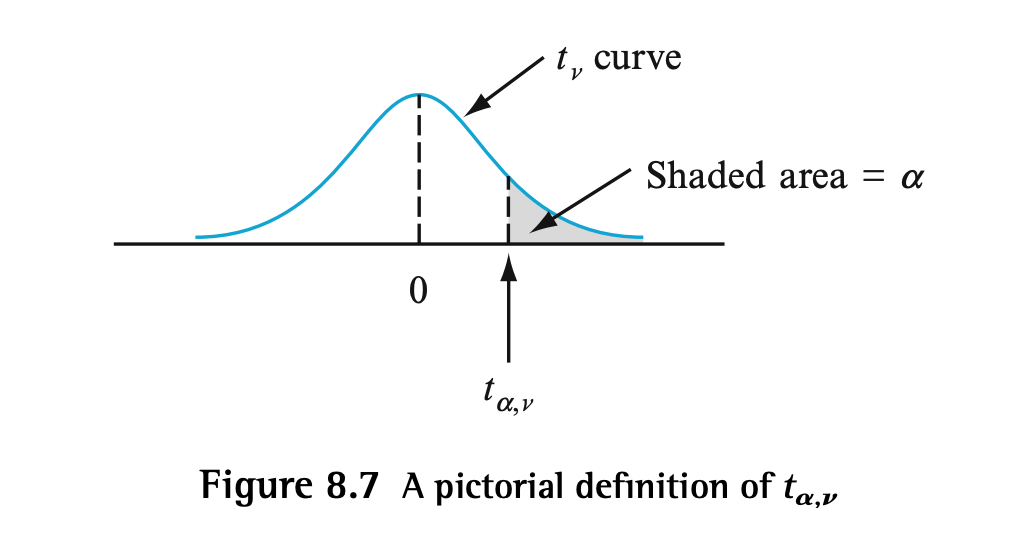
\includegraphics{images/criticalt.png}

Appendix A.5 shows the table with specific values of the t-distribution.
\end{frame}

\begin{frame}{Exercise 30}
\protect\hypertarget{exercise-30}{}
Determine the \(t\) critical value that will capture the desired \(t\)
curve area in each of the following cases:

\begin{enumerate}[<+->]
[a.]
\tightlist
\item
  Central area = 0.95, df = 10
\item
  Central area = 0.95, df = 20
\item
  Central area = 0.99, df = 20
\item
  Central area = 0.99, df = 50
\item
  Upper-tail area = 0.01, df = 25
\item
  Lower-tail area = 0.025, df = 5
\end{enumerate}
\end{frame}

\begin{frame}{Exercise 30 Solutions}
\protect\hypertarget{exercise-30-solutions}{}
\begin{enumerate}[<+->]
[a.]
\tightlist
\item
\end{enumerate}

\begin{figure}

{\centering 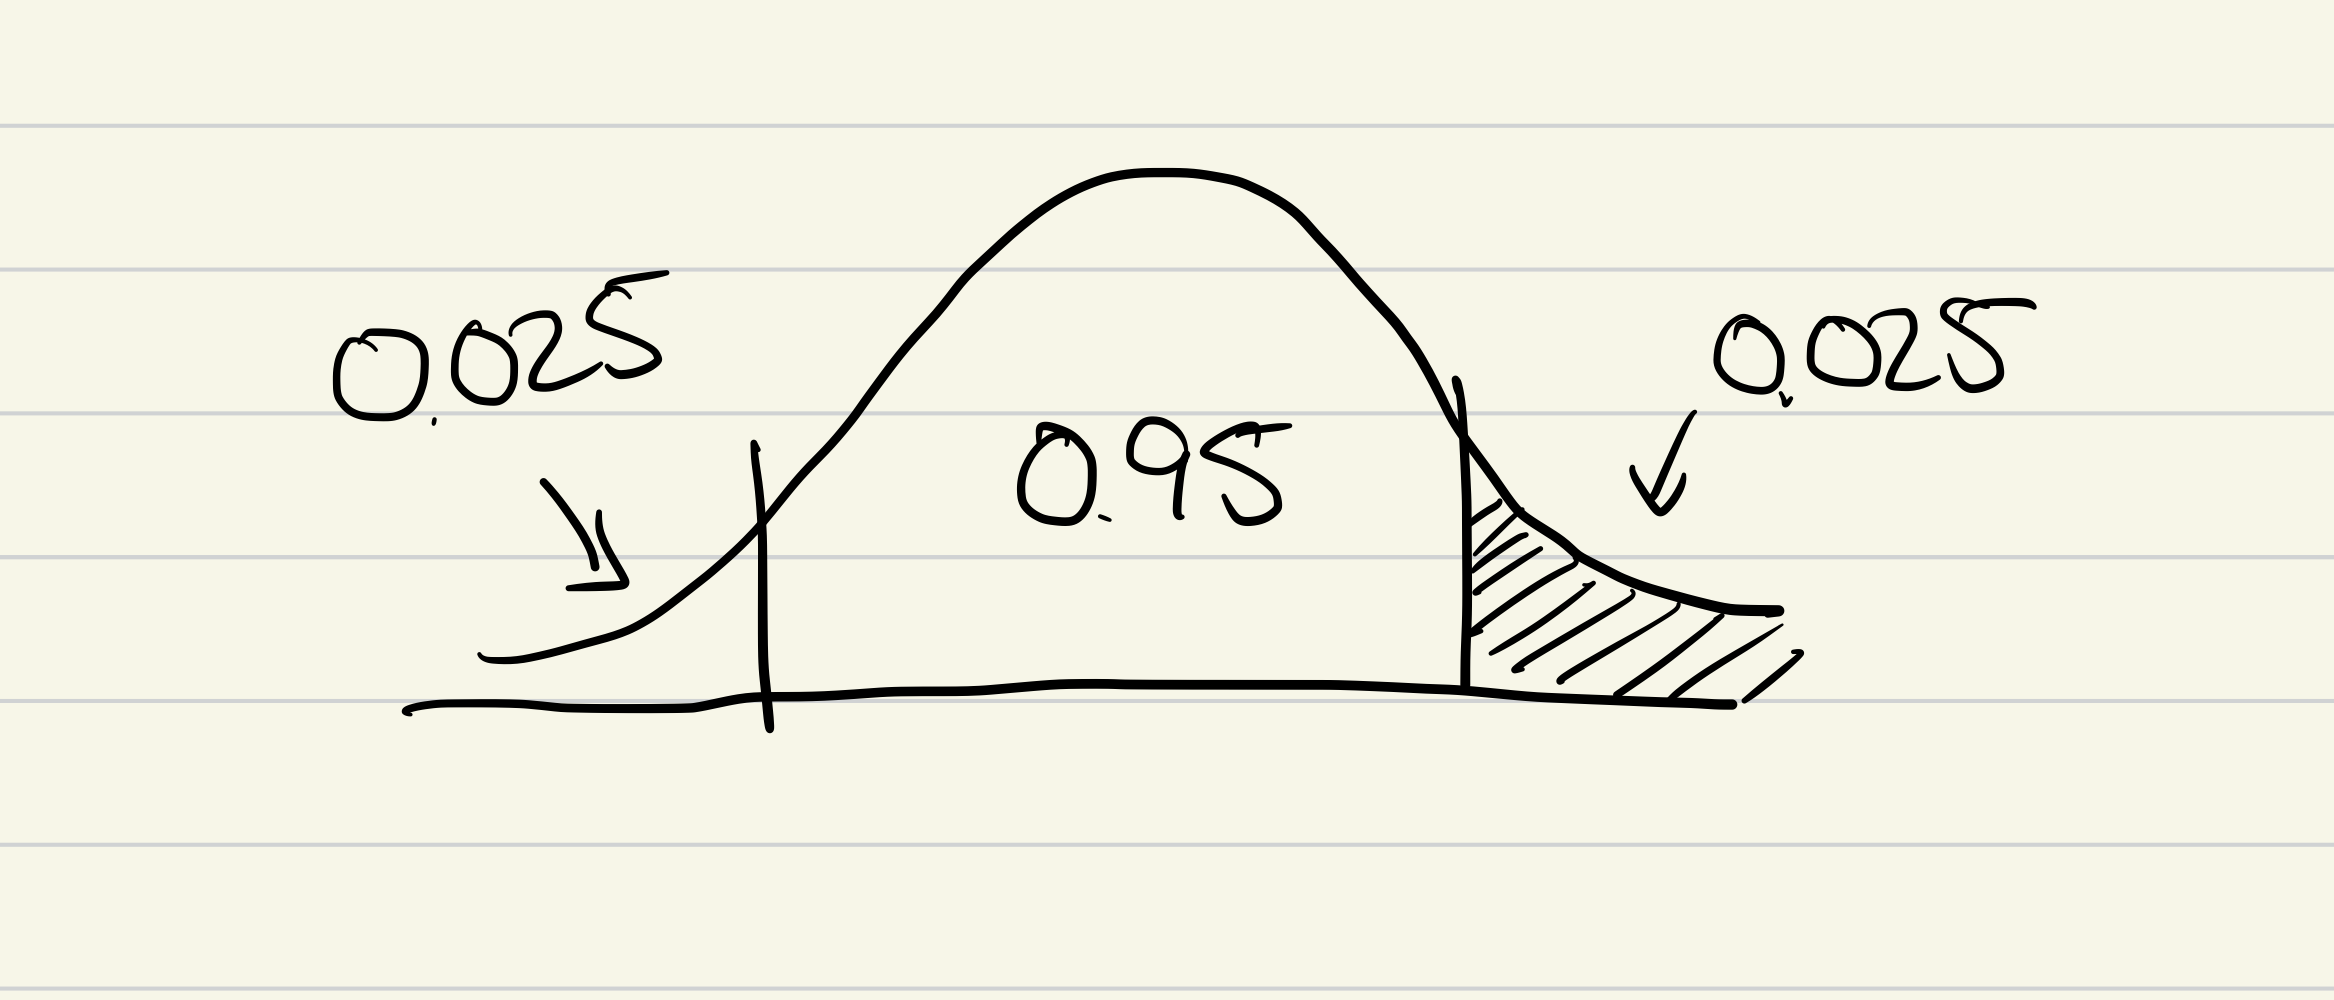
\includegraphics{images/central95.png}

}

\end{figure}

df = 10

From t-table, \(t = 2.228\)
\end{frame}

\begin{frame}{Exercise 30 Solutions}
\protect\hypertarget{exercise-30-solutions-1}{}
\begin{enumerate}[<+->]
[a.]
\setcounter{enumi}{1}
\tightlist
\item
\end{enumerate}

\begin{figure}

{\centering 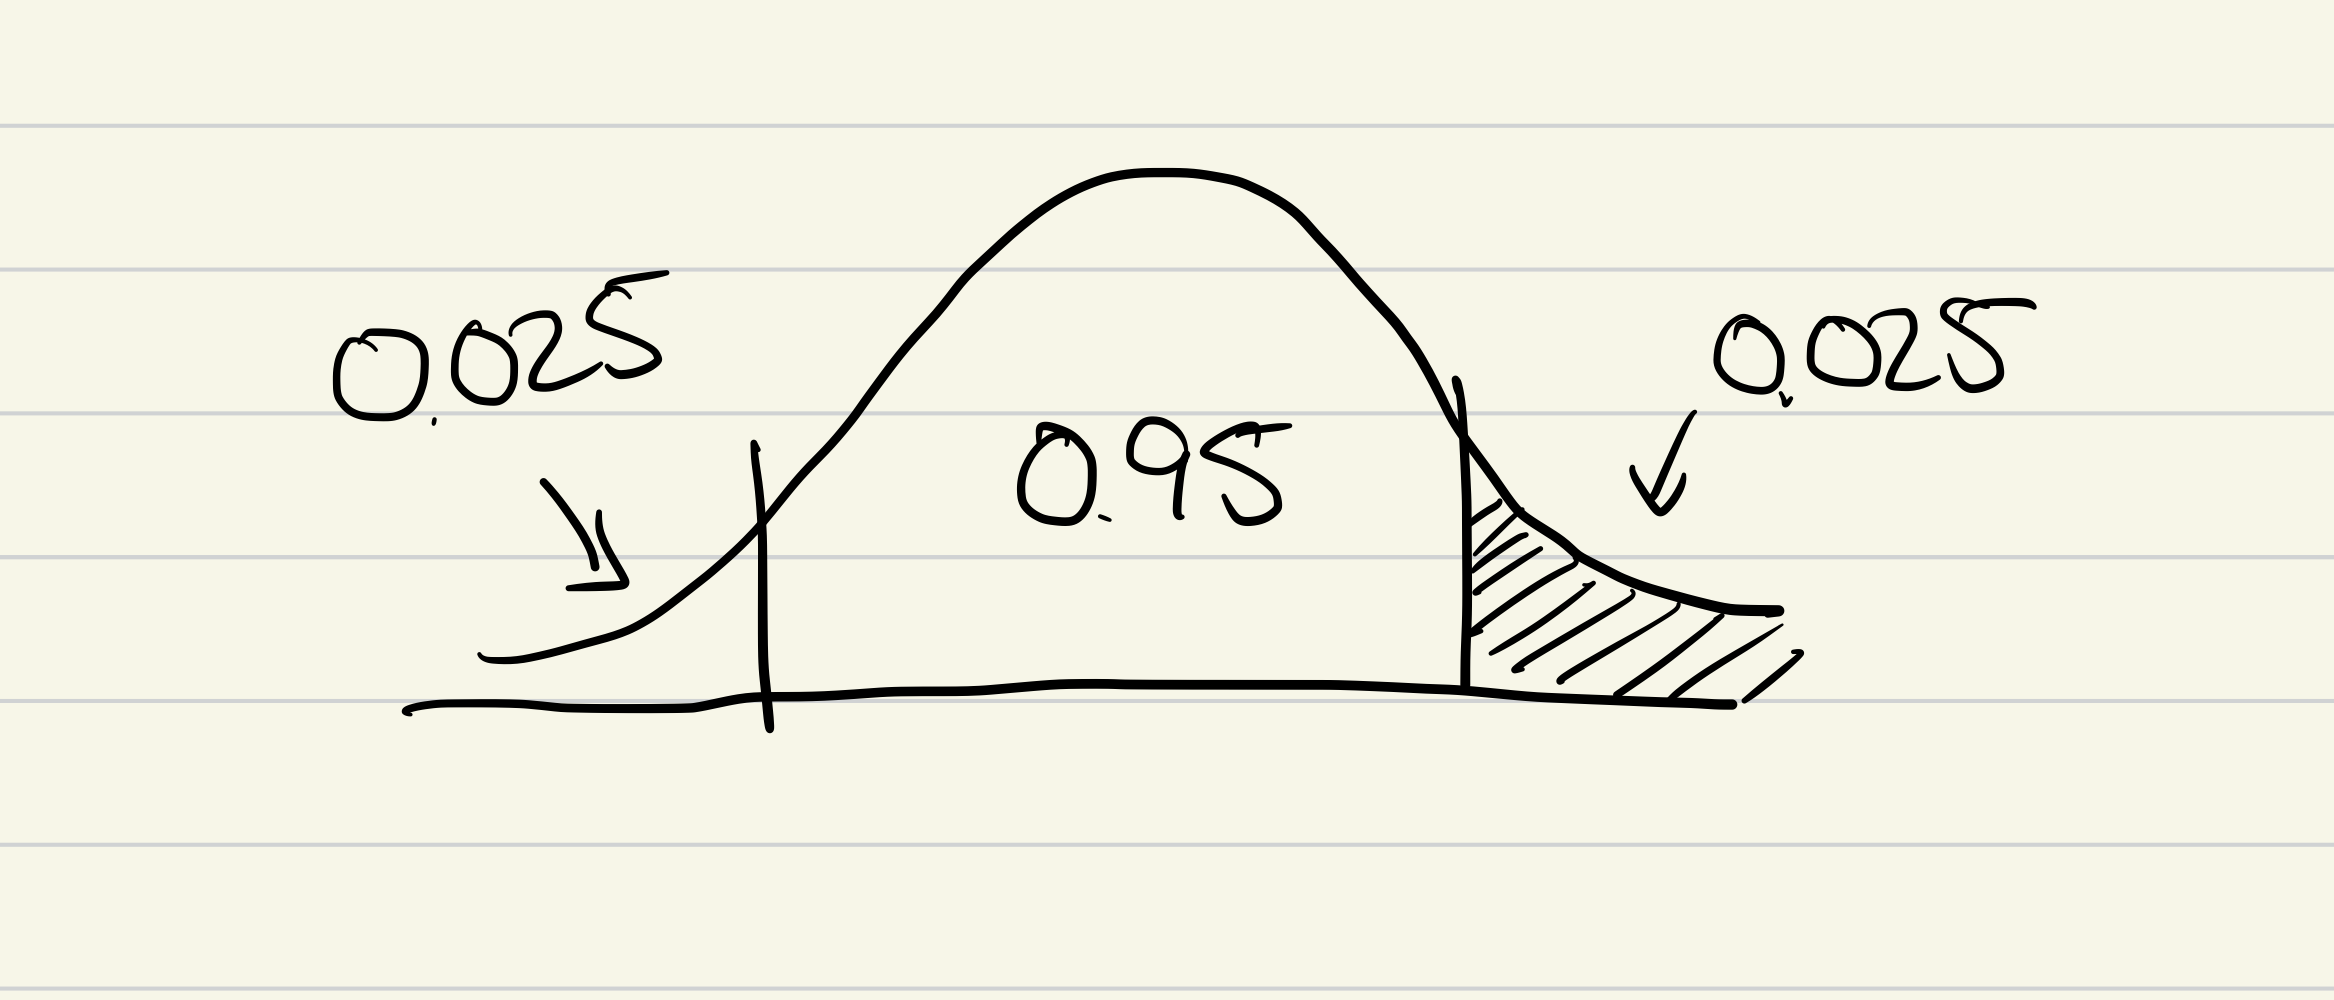
\includegraphics{images/central95.png}

}

\end{figure}

df = 20

From t-table, \(t = 2.086\)
\end{frame}

\begin{frame}{Exercise 30 Solutions}
\protect\hypertarget{exercise-30-solutions-2}{}
\begin{enumerate}[<+->]
[a.]
\setcounter{enumi}{2}
\tightlist
\item
\end{enumerate}

\begin{figure}

{\centering 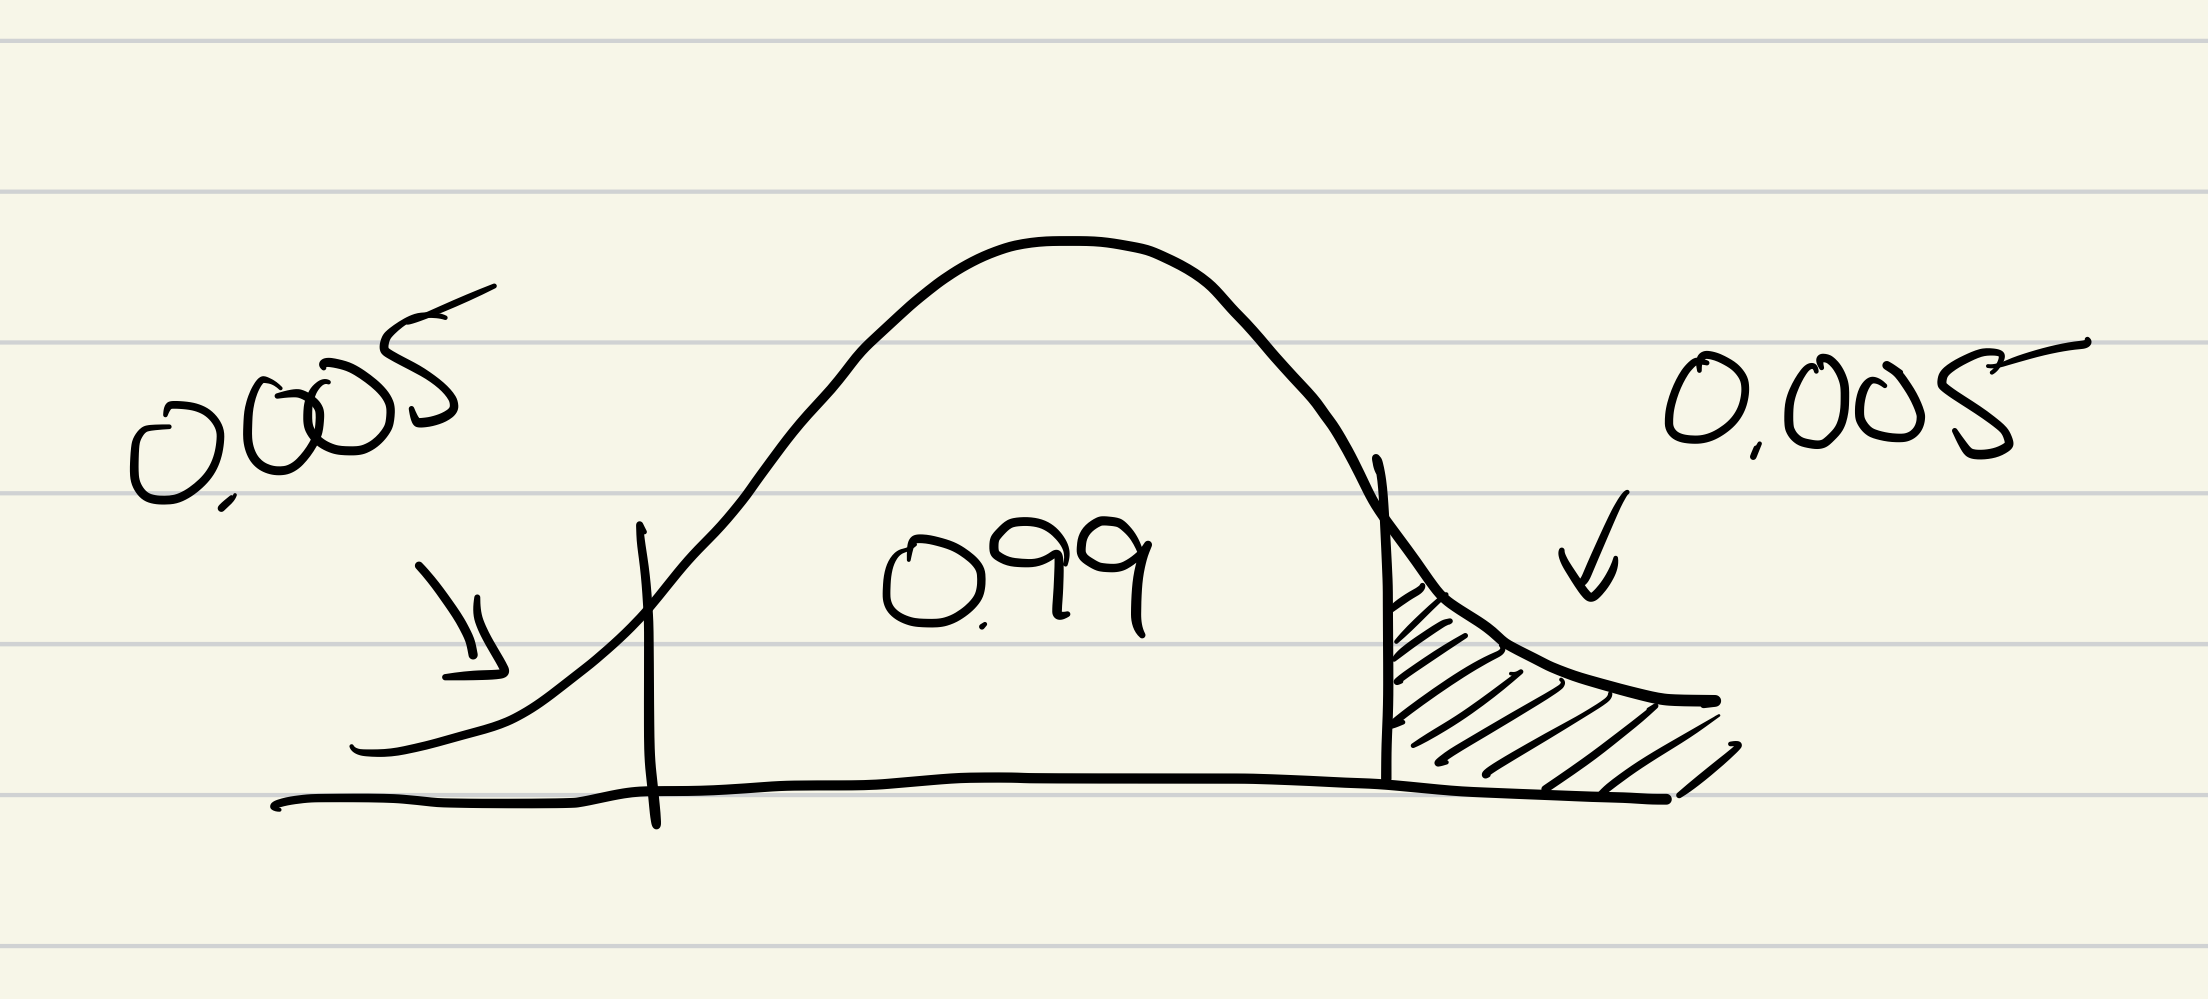
\includegraphics{images/central99-01.png}

}

\end{figure}

df = 20

From t-table, \(t = 2.845\)
\end{frame}

\begin{frame}{The one-sample t confidence interval}
\protect\hypertarget{the-one-sample-t-confidence-interval}{}
The standardized variable \(T\) has a \(t\) distribution with \(n-1\)
df, and the area under the corresponding \(t\) density curve between
\(-t_{\alpha/2,n-1}\) and \(t_{\alpha/2,n-1}\) is \(1-\alpha\) (area
\(\alpha/2\) lies in each tail), so

\[
P(-t_{\alpha/2;n-1} < T < t_{\alpha/2;n-1}) = 1 - \alpha
\]

This expression differs from expressions in previous sections in that
\(T\) and \(t_{\alpha/2,n-1}\) are used in place of \(Z\) and
\(z_{\alpha/2}\), but it can be manipulated in the same manner to obtain
a confidence interval for \(\mu\).
\end{frame}

\begin{frame}{The one-sample t confidence interval}
\protect\hypertarget{the-one-sample-t-confidence-interval-1}{}
\begin{tcolorbox}[enhanced jigsaw, titlerule=0mm, colbacktitle=quarto-callout-important-color!10!white, opacityback=0, bottomrule=.15mm, colback=white, colframe=quarto-callout-important-color-frame, arc=.35mm, title=\textcolor{quarto-callout-important-color}{\faExclamation}\hspace{0.5em}{Proposition}, toprule=.15mm, breakable, coltitle=black, leftrule=.75mm, bottomtitle=1mm, left=2mm, rightrule=.15mm, toptitle=1mm, opacitybacktitle=0.6]

Let \(\bar{x}\) and \(s\) be the sample mean and sample standard
deviation computed from the results of a random sample from a normal
distribution with mean \(\mu\). Then a
\textbf{100(1-}\(\alpha\)\textbf{)\% confidence interval for} \(\mu\),
the \textbf{one sample t CI} is:

\[
\left( \bar{x} - t_{\alpha/2,n-1}\frac{s}{\sqrt{n}},  \bar{x} + t_{\alpha/2,n-1}\frac{s}{\sqrt{n}}\right)
\]

or more compactly, \(\bar{x} \pm t_{\alpha/2,n-1}\frac{s}{\sqrt{n}}\).

An \textbf{upper confidence bound for} \(\mu\) is

\[
 \bar{x} + t_{\alpha,n-1}\frac{s}{\sqrt{n}}
\]

and by replacing \(+\) with \(-\) in this latter expression gives a
\textbf{lower confidence bound for} \(\mu\)\}. Both have confidence
level 100(1-\(\alpha\))\%.

\end{tcolorbox}
\end{frame}

\begin{frame}{Exercise 34}
\protect\hypertarget{exercise-34}{}
Here is a sample of ACT scores (average of the Math, English, Social
Science, and Natural Science scores) for students taking college
freshman calculus:

\begin{longtable}[]{@{}lllllll@{}}
\toprule()
24.00 & 28.00 & 27.75 & 27.00 & 24.25 & 23.50 & 26.25 \\
\midrule()
\endhead
24.00 & 25.00 & 30.00 & 23.25 & 26.25 & 21.50 & 26.00 \\
28.00 & 24.50 & 22.50 & 28.25 & 21.25 & 19.75 & \\
\bottomrule()
\end{longtable}

\begin{enumerate}[<+->]
[a.]
\tightlist
\item
  Using an appropriate graph, see if it is plausible that the
  observations were selected from a normal distribution.
\end{enumerate}
\end{frame}

\begin{frame}[fragile]{Exercise 34}
\protect\hypertarget{exercise-34-1}{}
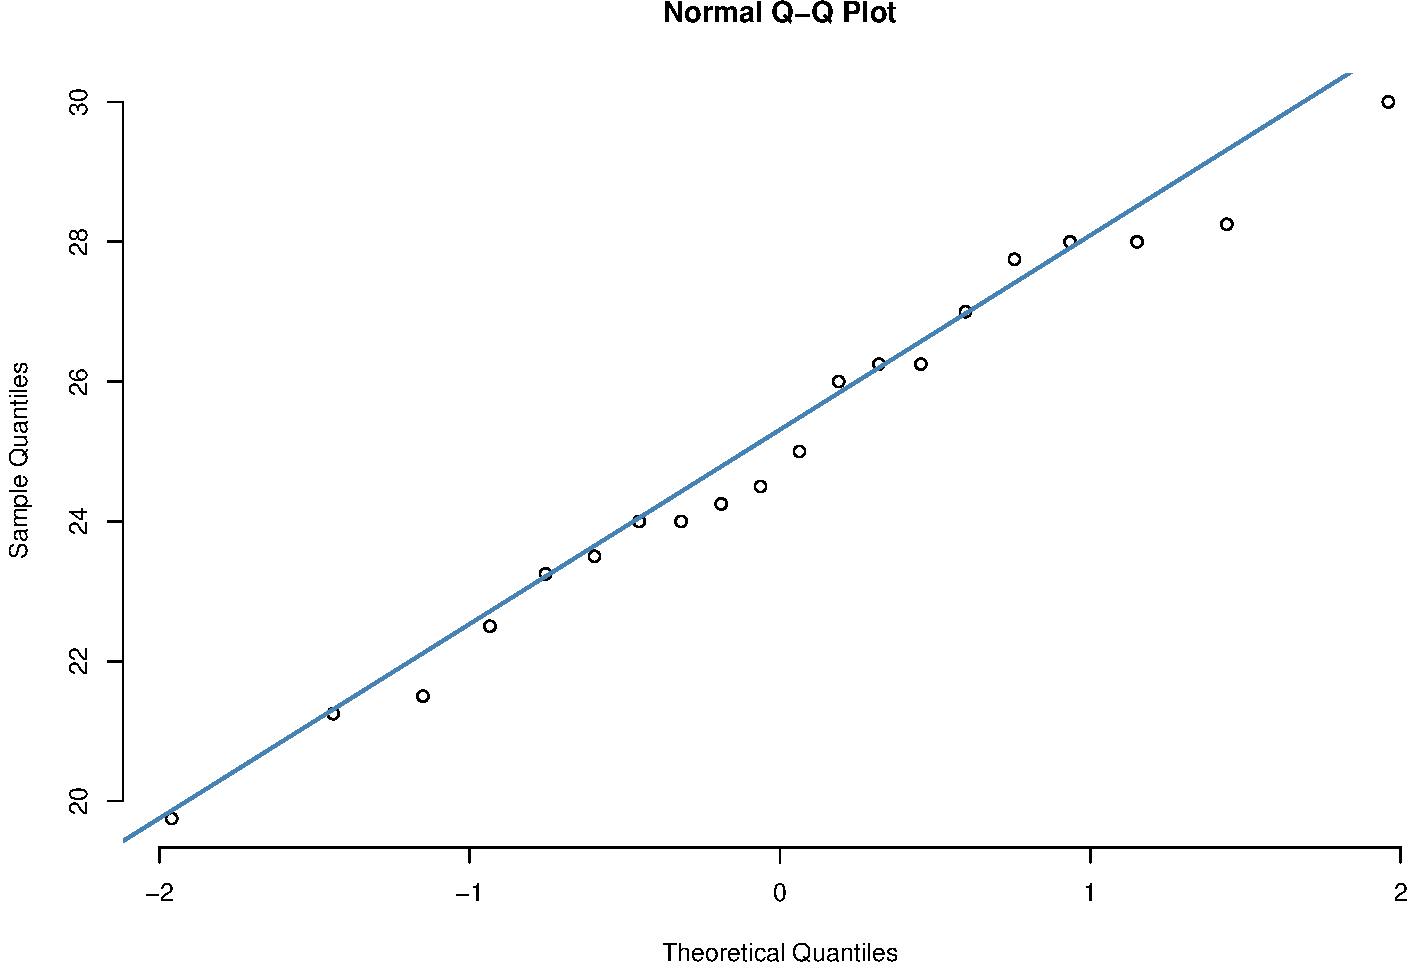
\includegraphics[width=0.5\textwidth,height=\textheight]{Chapter8Slides_files/figure-beamer/unnamed-chunk-1-1.pdf}

\begin{verbatim}
[1] "mean =  25.05"
\end{verbatim}

\begin{verbatim}
[1] "std =  2.68964877378363"
\end{verbatim}

\begin{verbatim}
[1] "n =  20"
\end{verbatim}
\end{frame}

\begin{frame}{Exercise 34}
\protect\hypertarget{exercise-34-2}{}
\begin{enumerate}[<+->]
[a.]
\setcounter{enumi}{1}
\tightlist
\item
  Calculate a two-sided 95\% confidence interval for the population
  mean.
\end{enumerate}

\[
\begin{aligned}
\bar{x} &\pm t_{\alpha/2,n-1}\frac{s}{\sqrt{n}} \\
25.05 &\pm 2.093 \frac{2.690}{\sqrt{20}} \\
25.05 &\pm 1.259 \\
(23.791&, 26.309)
\end{aligned}
\]

Therefore, we are 95\% confident that the true mean ACT score for
students taking college freshman calculus is between 23.791 and 26.309.
\end{frame}

\begin{frame}{Exercise 36}
\protect\hypertarget{exercise-36}{}
Even as traditional markets for sweetgum lumber have declined, large
section solid timbers traditionally used for construction bridges and
mats have become increasingly scarce. Below is data on the modulus of
rapture (psi).

\(\bar{x} = 7203.2\)\\
\(n = 30\)\\
\(s = 543.5\)

\begin{enumerate}[<+->]
[a.]
\setcounter{enumi}{1}
\tightlist
\item
  Estimate the true average modulus of rapture in a way that conveys
  information about precision and reliability.
\end{enumerate}
\end{frame}

\begin{frame}{Prediction Intervals}
\protect\hypertarget{prediction-intervals}{}
\begin{itemize}[<+->]
\tightlist
\item
  In many applications, an investigator wishes to \emph{predict} a
  single value of a variable to be observed at some future time, rather
  than to \emph{estimate} the mean value of that variable.
\item
  A \emph{point prediction} is analogous to a \emph{point estimate}, so
  for this situation, it is just \(\bar{x}\).
\item
  We have a random sample \(X_{1}\), \(X_{2}\),\ldots,\(X_{n}\) from a
  normal population distribution, and we wish to predict the value of
  \(X_{n+1}\), a single future observation.
\item
  A point predictor is \(\bar{X}\), and the resulting prediction error
  is \(\bar{X} - X_{n+1}\).
\end{itemize}
\end{frame}

\begin{frame}{Prediction Intervals}
\protect\hypertarget{prediction-intervals-1}{}
\begin{itemize}[<+->]
\tightlist
\item
  The expected value of the prediction error is:
\end{itemize}

\[
E(\bar{X} - X_{n+1}) = E(\bar{X}) - E(X_{n+1}) = \mu - \mu = 0
\]

\begin{itemize}[<+->]
\tightlist
\item
  Since \(X_{n+1}\) is independent of \(X_{1}\),\ldots,\(X_{n}\), it is
  independent of \(\bar{X}\), so the variance of the prediction error is
\end{itemize}

\[
V(\bar{X} - X_{n+1}) = V(\bar{X}) + V(X_{n+1}) = \frac{\sigma^{2}}{n} + \sigma^{2} = \sigma^{2}\left(1 + \frac{1}{n}\right)
\]
\end{frame}

\begin{frame}{Prediction Interval}
\protect\hypertarget{prediction-interval}{}
\begin{itemize}[<+->]
\tightlist
\item
  The prediction error is a linear combination of independent normally
  distributed rv's, so itself is normally distributed. Thus
\end{itemize}

\[
Z = \frac{(\bar{X} - X_{n+1}) - 0}{\sqrt{\sigma^{2}\left(1 + \frac{1}{n}\right)}} = \frac{\bar{X} - X_{n+1}}{\sqrt{\sigma^{2}\left(1 + \frac{1}{n}\right)}}
\]

has a standard normal distribution.

\begin{itemize}[<+->]
\tightlist
\item
  As in the derivation of the distribution of
  \((\bar{X} - \mu)/(S/\sqrt{n})\), it can be shown that replacing
  \(\sigma\) by the sample standard deviation \(S\) (of
  \(X_{1}\),\ldots.,\(X_{n}\)) results in
\end{itemize}

\[
T = \frac{\bar{X} - X_{n+1}}{S\sqrt{1 + \frac{1}{n}}} \sim t \text{ distribution with } n - 1 \text{ df }
\]

\begin{itemize}[<+->]
\tightlist
\item
  Manipulating this \(T\) variable gives the following results.
\end{itemize}
\end{frame}

\begin{frame}{Prediction Interval for a Single Future Value}
\protect\hypertarget{prediction-interval-for-a-single-future-value}{}
\begin{tcolorbox}[enhanced jigsaw, titlerule=0mm, colbacktitle=quarto-callout-important-color!10!white, opacityback=0, bottomrule=.15mm, colback=white, colframe=quarto-callout-important-color-frame, arc=.35mm, title=\textcolor{quarto-callout-important-color}{\faExclamation}\hspace{0.5em}{Proposition}, toprule=.15mm, breakable, coltitle=black, leftrule=.75mm, bottomtitle=1mm, left=2mm, rightrule=.15mm, toptitle=1mm, opacitybacktitle=0.6]

A \textbf{prediction interval (PI)} for a single observation to be
selected from a normal population distribution is

\[
\bar{x} \pm t_{\alpha/2,n-1}\cdot s\sqrt{1 + \frac{1}{n}}
\]

The \textbf{prediction level} is 100(1-\(\alpha\))\%.

\end{tcolorbox}

Interpretation: if the interval is calculated sample after sample, in
the long run, 95\% of these intervals will include the corresponding
future values of \(X\).
\end{frame}

\begin{frame}{Exercise 34}
\protect\hypertarget{exercise-34-3}{}
Consider the ACT scores for students taking college freshman calculus
again.

Predict the ACT score for a single student taking college freshman
calculus in a way that conveys information about precision and
reliability. How does the resulting prediction compare to the estimate
we found before?

\[
\begin{aligned}
\bar{x} &\pm t_{\alpha/2,n-1}\cdot s\sqrt{1 + \frac{1}{n}} \\
25.05 &\pm 2.093 \cdot 2.690\sqrt{1 + \frac{1}{20}} \\
25.05 &\pm 5.769\\
(19.281&, 30.819)
\end{aligned}
\]
\end{frame}

\begin{frame}{Exercise 34 Solutions}
\protect\hypertarget{exercise-34-solutions}{}
\begin{itemize}[<+->]
\tightlist
\item
  I predict with 95\% confidence that the next student taking college
  freshman calculus will have an ACT score between 19.281 and 30.819.
\item
  This interval is wider than the confidence interval for \(\mu\) to
  account for the higher variability of an individual compared to a
  mean.
\end{itemize}
\end{frame}

\begin{frame}{Exercise 36}
\protect\hypertarget{exercise-36-1}{}
Even as traditional markets for sweetgum lumber have declined, large
section solid timbers traditionally used for construction bridges and
mats have become increasingly scarce. Below is data on the modulus of
rapture (psi).

\(\bar{x} = 7203.2\)\\
\(n = 30\)\\
\(s = 543.5\)

\begin{enumerate}[<+->]
[a.]
\setcounter{enumi}{2}
\tightlist
\item
  Predict the modulus for a single beam in a way that conveys
  information about precision and reliability. How does the resulting
  prediction compare to the estimate in (b).
\end{enumerate}
\end{frame}

\begin{frame}{Intervals Based on Nonnormal Population Distributions}
\protect\hypertarget{intervals-based-on-nonnormal-population-distributions}{}
\begin{itemize}[<+->]
\tightlist
\item
  The one sample \(t\) CI for \(\mu\) is robust to small or even
  moderate departures from normality unless \(n\) is quite small.
\item
  That is, unless \(n\) is quite small and the departures from normality
  are extreme, the one sample \(t\) interval should yield coverage
  probabilities close to the nominal confidence level.
\item
  However, the prediction intervals are closely tied to the normality
  assumption. These intervals should not be used in the absence of
  compelling evidence for normality.
\end{itemize}
\end{frame}

\begin{frame}{Summary}
\protect\hypertarget{summary-4}{}
\begin{itemize}[<+->]
\tightlist
\item
  When \(\bar{X}\) is the mean of a random sample of size \(n\) from a
  normal population with mean \(\mu\), then
\end{itemize}

\[
T = \frac{\bar{X} - \mu}{S/\sqrt{n}}
\]

has the \(t\) distribution with \(n-1\) degrees of freedom.

\begin{itemize}[<+->]
\tightlist
\item
  Each \(t_{\nu}\) curve is bell-shaped and centered at 0.
\item
  Each \(t_{\nu}\) curve is more spread out than the standard normal (z)
  curve.
\item
  As \(\nu\) increases, the spread of the \(t_{\nu}\) curve decreases.
\item
  As \(\nu \rightarrow \infty\), the sequence of \(t_{\nu}\) curves
  approach the standard normal curve.
\end{itemize}
\end{frame}

\begin{frame}{Summary}
\protect\hypertarget{summary-5}{}
\begin{itemize}[<+->]
\tightlist
\item
  \(t_{\alpha,\nu}\) = the number on the measurement axis for which the
  area under the \(t\) curve with \(\nu\) degrees of freedom to the
  right of \(t_{\alpha,\nu}\) is \(\alpha\). This is called a \textbf{t
  critical value}.
\item
  A 100(1-\(\alpha\))\% CI for \(\mu\), the one sample \(t\) CI, is
\end{itemize}

\[
\bar{x} \pm t_{\alpha/2,n-1}\cdot \frac{s}{\sqrt{n}}
\]

\begin{itemize}[<+->]
\tightlist
\item
  A 100(1-\(\alpha\))\% prediction interval (PI) for a single
  observation to be selected from a normal population distribution is
\end{itemize}

\[
\bar{x} \pm t_{\alpha/2,n-1}\cdot s\sqrt{1 + \frac{1}{n}}
\]
\end{frame}

\begin{frame}{Practice Problems}
\protect\hypertarget{practice-problems-2}{}
\begin{itemize}[<+->]
\tightlist
\item
  Odd problems 8.29 - 8.43
\end{itemize}
\end{frame}

\hypertarget{confidence-intervals-for-the-variance-and-standard-deviation-of-a-normal-population}{%
\section{8.4 Confidence Intervals for the Variance and Standard
Deviation of a Normal
Population}\label{confidence-intervals-for-the-variance-and-standard-deviation-of-a-normal-population}}

\begin{frame}{Outcomes}
\protect\hypertarget{outcomes-3}{}
By the end of this section, you will be able to

\begin{itemize}[<+->]
\tightlist
\item
  Be familiar with the chi-squared distribution, it's properties and
  know how to look up appropriate values using the table.
\item
  Know what random variable involving sample variance follows the
  chi-squared distribution.
\item
  Calculate a confidence interval for the population variance of a
  normal distribution and interpret.
\item
  Calculate a confidence interval for the population standard deviation
  of a normal distribution and interpret.
\end{itemize}
\end{frame}

\begin{frame}{Chi-Squared (\(\chi^{2}\)) Distribution}
\protect\hypertarget{chi-squared-chi2-distribution}{}
\begin{tcolorbox}[enhanced jigsaw, titlerule=0mm, colbacktitle=quarto-callout-important-color!10!white, opacityback=0, bottomrule=.15mm, colback=white, colframe=quarto-callout-important-color-frame, arc=.35mm, title=\textcolor{quarto-callout-important-color}{\faExclamation}\hspace{0.5em}{Definition}, toprule=.15mm, breakable, coltitle=black, leftrule=.75mm, bottomtitle=1mm, left=2mm, rightrule=.15mm, toptitle=1mm, opacitybacktitle=0.6]

Let \(\nu\) be a positive integer. Then a random variable \(X\) is said
to have a \textbf{chi-squared distribution} with parameter \(\nu\) if
the pdf of \(X\) is the gamma density with \(\alpha = \nu/2\) and
\(\beta=2\). The pdf of a chi-squared rv is thus

\[ 
f(x;\nu) = \begin{cases}
\frac{1}{2^{\nu/2}\Gamma(\nu/2)}x^{(\nu/2)-1}e^{-x/2} & x \geq 0 \\
0 & x < 0 
\end{cases}
\]

The parameter \(\nu\) is called the \textbf{number of degrees of freedom
(df)} of X. The symbol \(\chi^{2}\) is often used in place of
``chi-squared''.

\end{tcolorbox}
\end{frame}

\begin{frame}{Chi-Squared (\(\chi^{2}\)) Distribution}
\protect\hypertarget{chi-squared-chi2-distribution-1}{}
\begin{tcolorbox}[enhanced jigsaw, titlerule=0mm, colbacktitle=quarto-callout-important-color!10!white, opacityback=0, bottomrule=.15mm, colback=white, colframe=quarto-callout-important-color-frame, arc=.35mm, title=\textcolor{quarto-callout-important-color}{\faExclamation}\hspace{0.5em}{Proposition}, toprule=.15mm, breakable, coltitle=black, leftrule=.75mm, bottomtitle=1mm, left=2mm, rightrule=.15mm, toptitle=1mm, opacitybacktitle=0.6]

If Z has a standard normal distribution and \(X = Z^{2}\), then the pdf
of X is

\[
f(x;\nu) = \begin{cases}
\frac{1}{2^{1/2}\Gamma(1/2)}x^{(1/2)-1}e^{-x/2} & x \geq 0 \\
0 & x < 0 
\end{cases}
\]

That is, X is chi-squared with 1 df, \(X \sim \chi^{2}_{1}\).

\end{tcolorbox}
\end{frame}

\begin{frame}{Chi-Squared (\(\chi^{2}\)) Distribution}
\protect\hypertarget{chi-squared-chi2-distribution-2}{}
\begin{tcolorbox}[enhanced jigsaw, titlerule=0mm, colbacktitle=quarto-callout-important-color!10!white, opacityback=0, bottomrule=.15mm, colback=white, colframe=quarto-callout-important-color-frame, arc=.35mm, title=\textcolor{quarto-callout-important-color}{\faExclamation}\hspace{0.5em}{Proposition}, toprule=.15mm, breakable, coltitle=black, leftrule=.75mm, bottomtitle=1mm, left=2mm, rightrule=.15mm, toptitle=1mm, opacitybacktitle=0.6]

If \(X_{1} \sim \chi^{2}_{\nu_{1}}\), \(X_{2} \sim \chi^{2}_{\nu_{2}}\)
and they are independent, then
\(X_{1} + X_{2} \sim \chi^{2}_{\nu_{1} + \nu_{2}}\)

\end{tcolorbox}

\begin{tcolorbox}[enhanced jigsaw, titlerule=0mm, colbacktitle=quarto-callout-important-color!10!white, opacityback=0, bottomrule=.15mm, colback=white, colframe=quarto-callout-important-color-frame, arc=.35mm, title=\textcolor{quarto-callout-important-color}{\faExclamation}\hspace{0.5em}{Proposition}, toprule=.15mm, breakable, coltitle=black, leftrule=.75mm, bottomtitle=1mm, left=2mm, rightrule=.15mm, toptitle=1mm, opacitybacktitle=0.6]

If \(Z_{1}\), \(Z_{2}\),\ldots,\(z_{n}\) are independent and each has
the standard normal distribution, then
\(Z_{1}^{2} + Z_{2}^{2} + \cdots + Z_{n}^{2} \sim \chi^{2}_{n}\)

\end{tcolorbox}

\begin{tcolorbox}[enhanced jigsaw, titlerule=0mm, colbacktitle=quarto-callout-important-color!10!white, opacityback=0, bottomrule=.15mm, colback=white, colframe=quarto-callout-important-color-frame, arc=.35mm, title=\textcolor{quarto-callout-important-color}{\faExclamation}\hspace{0.5em}{Proposition}, toprule=.15mm, breakable, coltitle=black, leftrule=.75mm, bottomtitle=1mm, left=2mm, rightrule=.15mm, toptitle=1mm, opacitybacktitle=0.6]

If \(X_{1}\),\ldots,\(X_{n}\) are a random sample from a normal
distribution, then \(\bar{X}\) and \(S^{2}\) are independent.

\end{tcolorbox}

\begin{tcolorbox}[enhanced jigsaw, titlerule=0mm, colbacktitle=quarto-callout-important-color!10!white, opacityback=0, bottomrule=.15mm, colback=white, colframe=quarto-callout-important-color-frame, arc=.35mm, title=\textcolor{quarto-callout-important-color}{\faExclamation}\hspace{0.5em}{Proposition}, toprule=.15mm, breakable, coltitle=black, leftrule=.75mm, bottomtitle=1mm, left=2mm, rightrule=.15mm, toptitle=1mm, opacitybacktitle=0.6]

If \(X_{3} = X_{1} + X_{2}\), and \(X_{1} \sim \chi^{2}_{\nu_{1}}\),
\(X_{3} \sim \chi^{2}_{\nu_{3}}\), and \(X_{1}\), and \(X_{2}\) are
independent, then \(X_{2} \sim \chi^{2}_{\nu_{3} - \nu_{1}}\)

\end{tcolorbox}
\end{frame}

\begin{frame}{Distribution of Sample Variance}
\protect\hypertarget{distribution-of-sample-variance}{}
\begin{tcolorbox}[enhanced jigsaw, titlerule=0mm, colbacktitle=quarto-callout-important-color!10!white, opacityback=0, bottomrule=.15mm, colback=white, colframe=quarto-callout-important-color-frame, arc=.35mm, title=\textcolor{quarto-callout-important-color}{\faExclamation}\hspace{0.5em}{Theorem}, toprule=.15mm, breakable, coltitle=black, leftrule=.75mm, bottomtitle=1mm, left=2mm, rightrule=.15mm, toptitle=1mm, opacitybacktitle=0.6]

If \(X_{1}\), \(X_{2}\),\ldots,\(X_{n}\) are a random sample from a
normal distribution with parameters \(\mu\) and \(\sigma^{2}\). Then the
rv

\[
\frac{(n-1)S^{2}}{\sigma^{2}} = \frac{\sum(X_{i}-\bar{X})^{2}}{\sigma^{2}}
\]

has a chi-squared (\(\chi^{2}_{n-1}\)) distribution with \(n-1\) df.

\end{tcolorbox}

Let's prove it!
\end{frame}

\begin{frame}{Chi-Squared Critical Value}
\protect\hypertarget{chi-squared-critical-value}{}
\begin{tcolorbox}[enhanced jigsaw, titlerule=0mm, colbacktitle=quarto-callout-important-color!10!white, opacityback=0, bottomrule=.15mm, colback=white, colframe=quarto-callout-important-color-frame, arc=.35mm, title=\textcolor{quarto-callout-important-color}{\faExclamation}\hspace{0.5em}{Notation}, toprule=.15mm, breakable, coltitle=black, leftrule=.75mm, bottomtitle=1mm, left=2mm, rightrule=.15mm, toptitle=1mm, opacitybacktitle=0.6]

Let \(\chi^{2}_{\alpha,\nu}\), called a \textbf{chi-squared critical
value}, denote the number on the measurement axis such that \(\alpha\)
of the area under the chi-squared curve with \(\nu\) df lies to the
right of \(\chi^{2}_{\alpha,\nu}\).

\end{tcolorbox}

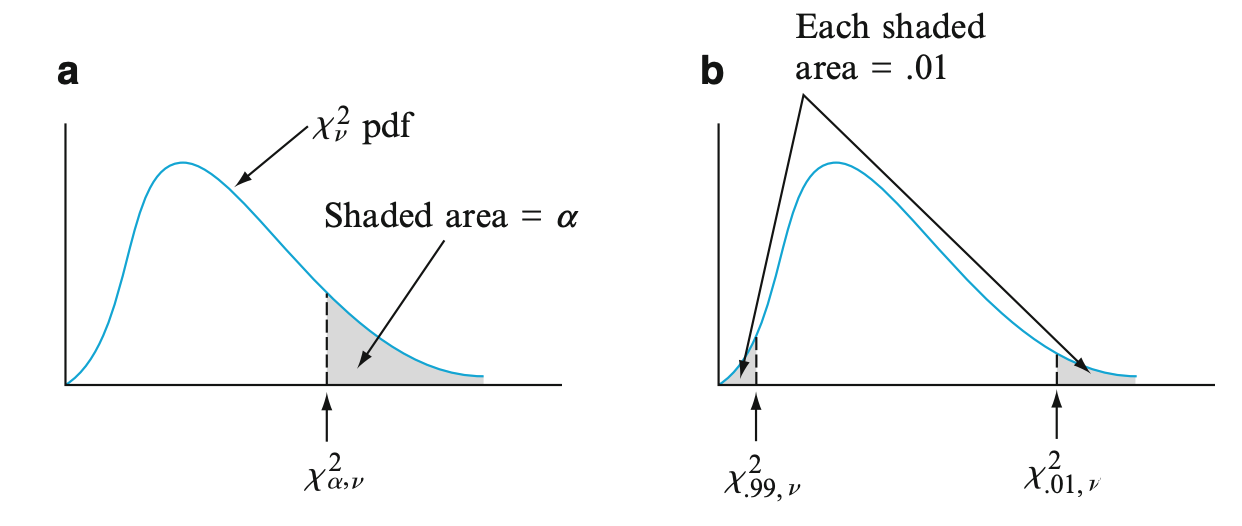
\includegraphics{images/notation.png}
\end{frame}

\begin{frame}{Exercise 44}
\protect\hypertarget{exercise-44}{}
Determine the values of the following quantities

\begin{enumerate}[<+->]
[a.]
\tightlist
\item
  \(\chi^{2}_{0.1,15}\)
\end{enumerate}

Looking up in the \(\chi^{2}\) table for \(\alpha = 0.1\) and
\(\nu = 15\), we find \(\chi^{2}_{0.1,15} = 22.307\).

\begin{enumerate}[<+->]
[a.]
\setcounter{enumi}{1}
\tightlist
\item
  \(\chi^{2}_{0.1, 25}\)
\end{enumerate}

Looking up in the \(\chi^{2}\) table for \(\alpha = 0.1\) and
\(\nu = 25\), we find \(\chi^{2}_{0.1,25} = 34.381\).

\begin{enumerate}[<+->]
[a.]
\setcounter{enumi}{2}
\tightlist
\item
  \(\chi^{2}_{0.01,25}\)
\end{enumerate}

Looking up in the \(\chi^{2}\) table for \(\alpha = 0.01\) and
\(\nu = 25\), we find \(\chi^{2}_{0.01,25} = 44.313\).
\end{frame}

\begin{frame}{Exercise 44}
\protect\hypertarget{exercise-44-1}{}
\begin{enumerate}[<+->]
[a.]
\setcounter{enumi}{3}
\tightlist
\item
  \(\chi^{2}_{0.005, 25}\)
\item
  \(\chi^{2}_{0.99, 25}\)
\item
  \(\chi^{2}_{0.995, 25}\)
\end{enumerate}
\end{frame}

\begin{frame}{Confidence intervals for \(\sigma^{2}\)}
\protect\hypertarget{confidence-intervals-for-sigma2}{}
\begin{itemize}[<+->]
\tightlist
\item
  The rv \((n-1)S^{2}/\sigma^{2}\) satisfies the two properties on which
  the general method for obtaining a CI is based: it is a function of
  the parameter of interest \(\sigma^{2}\), yet its probability
  distribution (chi-squared) does not depend on this parameter.
\item
  Therefore, we get:
\end{itemize}

\[
P\left( \chi^{2}_{1-\alpha/2,n-1} < \frac{(n-1)S^{2}}{\sigma^{2}} < \chi^{2}_{\alpha/2,n-1}\right) = 1-\alpha
\]

Rearranging the inequality, we get:

\[
\frac{(n-1)S^{2}}{\chi^{2}_{\alpha/2,n-1}} < \sigma^{2} < \frac{(n-1)S^{2}}{\chi^{2}_{1-\alpha/2,n-1}}
\]
\end{frame}

\begin{frame}{Confidence Interval for \(\sigma^{2}\)}
\protect\hypertarget{confidence-interval-for-sigma2}{}
\begin{tcolorbox}[enhanced jigsaw, titlerule=0mm, colbacktitle=quarto-callout-important-color!10!white, opacityback=0, bottomrule=.15mm, colback=white, colframe=quarto-callout-important-color-frame, arc=.35mm, title=\textcolor{quarto-callout-important-color}{\faExclamation}\hspace{0.5em}{CI}, toprule=.15mm, breakable, coltitle=black, leftrule=.75mm, bottomtitle=1mm, left=2mm, rightrule=.15mm, toptitle=1mm, opacitybacktitle=0.6]

a \textbf{100(1-}\(\alpha\))\% confidence interval for the variance
\(\sigma^{2}\) of a normal population has lower limit

\[
\frac{(n-1)s^{2}}{\chi^{2}_{\alpha/2,n-1}}
\]

and upper limit

\[
\frac{(n-1)s^{2}}{\chi^{2}_{1-\alpha/2,n-1}}
\]

A \textbf{confidence interval for} \(\sigma\) has lower and upper limits
that are the square roots of the corresponding limits in the interval
for \(\sigma^{2}\).

\end{tcolorbox}
\end{frame}

\begin{frame}{Exercise 46}
\protect\hypertarget{exercise-46}{}
Exercise 34 gave a random sample of 20 ACT scores from students taking
college freshman calculus. Calculate a 99\% CI for the standard
deviation of the population distribution. Is this interval valid
whatever the nature of the distribution? Explain.

\(s = 2.690\)\\
\(n = 20\)
\end{frame}

\begin{frame}{Exercise 46 Solutions}
\protect\hypertarget{exercise-46-solutions}{}
\[
\begin{aligned}
\frac{(n-1)s^{2}}{\chi^{2}_{\alpha/2,n-1}} < &\sigma^{2} < \frac{(n-1)s^{2}}{\chi^{2}_{1-\alpha/2,n-1}}\\
\frac{(20-1)2.690^{2}}{\chi^{2}_{0.01/2,20-1}} < &\sigma^{2} < \frac{(20-1)2.690^{2}}{\chi^{2}_{1-0.01/2,20-1}} \\
\frac{(19)2.690^{2}}{38.580} < &\sigma^{2} < \frac{(19)2.690^{2}}{6.843} \\
3.564 < &\sigma^{2} < 20.091
\end{aligned}
\]

So the interval for \(\sigma\) is
\((\sqrt{3.564}, \sqrt{20.091}) = (1.888, 4.482)\).

This interval estimate is only valid for normally distributed data,
which was verified earlier with this dataset.
\end{frame}

\begin{frame}{Exercise 48}
\protect\hypertarget{exercise-48}{}
Refer to the baseball game times in Exercise 41. Calculate an upper
confidence bound with confidence level 95\% for the population standard
deviation of game time. Interpret your interval.

\(s = 19.89\)\\
\(n = 63\)
\end{frame}

\begin{frame}{Summary}
\protect\hypertarget{summary-6}{}
\begin{itemize}[<+->]
\tightlist
\item
  \(\frac{(n-1)S^{2}}{\sigma^{2}}\) has a chi-squared distribution with
  \(n-1\) degrees of freedom if \(X_{1}\), \(X_{2}\),\ldots,\(X_{n}\) is
  a random sample from a normal population.
\item
  \(\chi^{2}_{\alpha,\nu}\) is the \textbf{chi-squared critical value}
  with upper tail area \(\alpha\) and \(\nu\) degrees of freedom.
\item
  A \textbf{100(1-}\(\alpha\))\% confidence interval for the variance
  \(\sigma^{2}\) of a normal population has lower limit
  \((n-1)s^{2}/\chi^{2}_{\alpha/2,n-1}\) and upper limit
  \((n-1)s^{2}/\chi^{2}_{1-\alpha/2,n-1}\).
\item
  A \textbf{confidence interval for} \(\sigma\) has lower and upper
  limits that are the square roots of the corresponding limits in the
  interval for \(\sigma^{2}\).
\end{itemize}
\end{frame}

\begin{frame}{Practice Problems}
\protect\hypertarget{practice-problems-3}{}
\begin{itemize}[<+->]
\tightlist
\item
  Odd problems 8.45 - 8.47
\end{itemize}
\end{frame}



\end{document}
